\documentclass[12pt, a4paper]{article}
\usepackage{listings}
\usepackage{sourcecodepro}
\usepackage{xcolor}
\definecolor{backcolour}{rgb}{0.95,0.95,0.92}
\definecolor{codegray}{rgb}{0.5,0.5,0.5}
\lstdefinestyle{mystyle}{
	backgroundcolor=\color{backcolour},   
	numberstyle=\tiny\color{codegray},
	keywordstyle=\color{black}\bfseries,
	breakatwhitespace=false,         
	breaklines=true,                 
	captionpos=b,                    
	keepspaces=true,                 
	numbers=left,                    
	numbersep=5pt,                  
	showspaces=false,                
	showstringspaces=false,
	showtabs=false,                  
	tabsize=2,
	basicstyle=\scriptsize\ttfamily
}
\lstset{style=mystyle}
\usepackage[dutch]{babel}
\usepackage{array}
\usepackage{adjustbox}
\usepackage{wrapfig}
\usepackage{stix}
\usepackage{amsmath}
\newcommand*{\ora}{\overrightarrow}
\usepackage{tikz}
\usepackage{tikz-3dplot}
\usetikzlibrary{3d}
\usepackage{pgfplots}
\usepackage{algorithm}
\usepackage[noend]{algpseudocode}
\usepackage{graphicx}
\usepackage{subfig}
\graphicspath{{images/}}
\usepackage{chngcntr}
\usetikzlibrary{calc}
\usetikzlibrary{angles}
\usepackage{fp}
\usepackage{float}
\counterwithin{figure}{section}
\usepackage{hyperref}
\usepackage{titlesec}
\title{\Huge SDF's vs. Polygonen:\\ \large Een vergelijking van rendertechnieken}
\author{Taeke Roukema}
\date{Februari 2023}


\begin{document}
\maketitle
\begin{abstract}
Raytracen met gebruik van SDF's en raymarching levert een significant voordeel op tegenover het beschrijven van dezelfde vormen met meshes van polygonen.
\end{abstract}
\clearpage
\tableofcontents{}
\clearpage
\section{Voorwoord}
\clearpage
\section{Inleiding}
\subsection{Introductie onderwerp}

Renderen is overal. Als je je telefoon opent zie je allerlei gerenderde vormen. Bij het ontbijt zijn verpakkingen volgeprint met teksten die met de computer getekend zijn. Als je langs een bouwterrein loopt zie je hyperrealistische visualisaties van de architectuur. Moderne blockbuster-films zitten tegenwoordig bomvol CGI\footnote{\textbf{C}omputer \textbf{G}enerated \textbf{I}magery}. En er zijn al tientallen jaren films te zien die helemaal door de computer gemaakt zijn. 

\begin{wrapfigure}{s}{0.5\textwidth}
    \includegraphics[width=1\linewidth]{toystory3comparison.jpg}
    \caption{Een frame uit Toy Story 3, aan de linkerkant worden geen lichtberekeningen gedaan, en aan de rechterkant wel.}
    \label{fig:toystory3}
\end{wrapfigure}

Voor Toy Story 3 (Figuur \ref{fig:toystory3}) werd er gemiddeld zeven uur over gedaan om een frame te renderen \cite{HowToyStory3WasMade}. En dat terwijl er gebruik werd gemaakt van twee gigantische render farms\footnote{Een computercluster speciaal gemaakt voor het renderen van CGI, de term was geïntroduceerd in de productie voor Bored Room\cite{MakingOfBoredRoom}}. Het renderen van films kost niet alleen enorm veel tijd, maar ook veel energie. Het is dus belangrijk dat het zo efficiënt mogelijk gebeurd. Er wordt over de hele wereld voortdurend onderzoek gedaan naar manieren om dit proces efficiënter te maken en te verbeteren. De opkomst van kunstmatige intelligentie begint al bewegingen te maken in de wereld van CGI \cite{NeRFactor}. Maar er wordt ook voortdurend voortuitgang gemaakt op fundamentelere manieren. Zo zijn er de afgelopen vijf jaar GPU's\footnote{\textbf{G}raphics \textbf{P}rocessing \textbf{U}nit} van Nvidia op de markt gekomen met ingebouwde support voor realtime raytracing\cite{NvidiaRTX}. Door op het hardware niveau de chips zo te ontwerpen dat ze heel goed zijn in bepaalde berekeningen die gebruikt worden voor het simuleren van licht kunnen GPU's gebruikt worden om voormalig minutendurende processen meer dan zestig keer per seconde uit te voeren. 
\begin{figure}[H]
    \centering
    \includegraphics[width=0.5\textwidth]{minecraftrtx.jpg}
    \caption{De videogame Minecraft kan gebruik maken van Nvidia GPU's om realtime lichtsimulaties te berekenen.}
    \label{fig:minecraftrtx}
\end{figure}

Er zijn twee belangrijke maatstaffen waarmee we de efficiëntie van een renderalgoritme kunnen meten. De eerste is vanzelfsprekend: snelheid. Als een frame sneller gerenderd is wordt er minder energie gebruikt en zijn we goedkoper uit. Maar ook geheugenbezetting is belangrijk om rekening mee te houden. Het geheugen is simpelweg de plaats in de computer waar alle informatie wordt opgeslagen. Als je berekeningen doet moet je ergens de resultaten tussendoor opslaan. Complexe scènes kunnen enorm veel details hebben, die allemaal in het geheugen opgeslagen zijn. Het is niet gratis om extra geheugen toe te voegen, het is dus belangrijk om de geheugenbezetting te minimaliseren. 

Vrijwel alles is tegenwoordig op een manier gerenderd. Objecten zijn gedesigned met gebruik van CAD\footnote{\textbf{C}omputer \textbf{A}ided \textbf{D}esign}. Besturingssytemen runnen op een grafische shell. En een meerendeel van advertenties gebruikt CGI.
% Beschrijven hoe renderen voorkomt in het dagelijkse leven

Volgens Peter Collinridge\cite{ScienceBehindPixarRendering} gebruikt de render farm van pixar 24000 processor cores verdeeld over 2000 computers. Er wordt dus waarschijnlijk gebruik gemaakt van computers met \(24000/2000=12\) cores. De Ryzen 9 5900x is een voorbeeld van een processor met 12 cores, het energiegebruik zal niet exact hetzelfde zijn maar het ligt bij elkaar in de buurt. De 5900x gebruikt 105 Watt. \(105W\cdot 2000\approx 2,10\cdot 10^5W\). Volgens dezelfde bron kostte het renderen van Monster's University twee jaar. Dat is \(2\cdot 365\cdot 24\approx17520h\). \[210kW \cdot 17520h\approx 3679200kWh\] Een gemiddeld huishouden in Nederland gebruikt 2479 kWh per jaar. Dit betekent dat het renderen van Monster's University \(3679200/2479\approx 1484\) huishoudens een jaar lang van energie had kunnen voorzien. En dat is alleen nog maar de processorkracht, er gaat ook nog energie naar de moederborden, het geheugen, de koeling en de harde schijven. Kortom, er valt een hoop te besparen.
% Beschrijven hoeveel energie renderen kan kosten
% Impact klimaat
\subsection{Onderzoeksvraag/deelvragen}
\subsubsection{Hoofdvraag WIP}
In welke situaties is raymarching een efficiëntere rendertechniek dan polygonaal renderen?

Vergelijking van twee rendermethoden in rendersnelheid en geheugenbezetting.

Vergelijking van raymarching en polygonaal renderen in rendersnelheid en geheugenbezetting.

Hoe wegen raymarching en polygonaal renderen tegen elkaar op in rendersnelheid en geheugenbezetting?
\subsubsection{Deelvragen WIP}
\begin{itemize}
\item{Hoe beschrijf je een driedimensionale vorm?}
\item{Hoe werkt raytracing?}
\item{Hoe werkt raymarching?}
\item{Hoe werkt rasterization?}
\item{Hoe beschrijf je een vorm zodat het gerenderd kan worden met raymarching?}
\item{Hoeveel geheugen neemt polygonaal renderen in?}
\item{Hoeveel geheugen neemt renderen met raymarching in?}
\item{Hoe snel is renderen met raymarching vergeleken met polygonaal renderen?}
\item{Hoe kan je met raymarching objecten modelleren?}
\end{itemize}
\clearpage
\section{Theorie}
\subsection{Wat is renderen?}
Renderen is niks meer dan een computer die vormen tekent. Mensen zijn voortdurend bezig met het interacteren met computers, en die interactie verloopt via het beeldscherm. Maar de computer kan uit zichzelf niet zomaar alles tekenen. Daar worden allemaal algoritmes voor gebruikt. Een voorbeeld van zo'n algoritme is het tekenen van een rechthoek. In pseudocode zou dat als volgt voorgesteld kunnen worden:
\begin{algorithm}
\caption{Rechthoek Algoritme}
\begin{algorithmic}[1]
\Procedure{DrawRectangle}{x1, x2, y1, y2}
    \For{$x \gets x1$ to $x2$}             
	    \For{$y \gets y1$ to $y2$}             
		\State $\text{draw pixel at }(x, y)$
	    \EndFor
    \EndFor
\EndProcedure
\end{algorithmic}
\end{algorithm}

Het algoritme beschouwt elke pixel die binnen de rechthoek valt en kleurt die pixel. In dit geval wordt dat gedaan door twee loops, die samen alle mogelijke combinaties van x- en y-coördinaten doorlopen. 

Renderen omvat, in principe, niks anders dan het aansturen van individuele pixels. Zo'n pixel heeft op de meeste moderne beeldschermen drie waarden die de kleur aansturen: R, G en B, die respectievelijk staan voor rood, groen en blauw. Ze kunnen een geheel getal tussen de 0 en 255 aannemen wat resulteert in \(2^{24}\) mogelijke kleuren.
\begin{figure}[H]
\centering
\includegraphics[width=0.5\textwidth]{RGB_channels_separation.png}
\caption{De kleuren in een foto kunnen opgesplitst worden in rode, groene en blauwe kanalen.}
\label{fig:rgb_separated}
\end{figure}

Renderen gebeurt op een twee-dimensionaal beeldscherm. Dat betekent dat de positie van elke pixel te beschrijven is met twee waarden. Maar de wereld om ons heen kent niet twee, maar drie ruimtelijke dimensies. Door licht dat op ons netvlies valt na weerkaatst te zijn door verschillende objecten kunnen wij die wereld representeren in onze hersenen op een tweedimensionale manier. Camera's gebruiken een gelijksoortige techniek, de lens neemt het licht op en projecteert het op een sensor die de intensiteit en de kleur waarneemt. Met het renderen van driedimensionale objecten worden deze processen nagebootst. 

\subsection{Wat is realistisch?}
Het ligt nog niet zo voor de hand wanneer een door de computer gegenereerde afbeelding realistisch is, en wanneer niet. Gelukkig is de natuurkunde van licht in het dagelijks leven vrij simpel. In 1986 is de \textit{rendering equation} bedacht, die vrijwel al het gedrag van licht beschrijft \cite{RenderingEquation}.
\[
L_{\text{o}}(\mathbf x, \omega_{\text{o}}, \lambda, t) = L_{\text{e}}(\mathbf x, \omega_{\text{o}}, \lambda, t) \ + \int_\Omega f_{\text{r}}(\mathbf x, \omega_{\text{i}}, \omega_{\text{o}}, \lambda, t) L_{\text{i}}(\mathbf x, \omega_{\text{i}}, \lambda, t) (\omega_{\text{i}}\cdot\mathbf n) \operatorname d \omega_{\text{i}}
\]

Deze vergelijking oogt ingewikkeld, maar is in de werkelijkheid goed te overzien. 
\begin{itemize}
	\item $L_{\text{o}}(\mathbf x, \omega_{\text{o}}, \lambda, t)$ staat voor de uitkomende stralen licht
	\item $L_{\text{e}}(\mathbf x, \omega_{\text{o}}, \lambda, t)$ staat voor het uitgezonden licht van het object
	\item $	f_{\text{r}}(\mathbf x, \omega_{\text{i}}, \omega_{\text{o}}, \lambda, t)$ staat voor de materiaaleigenschappen van het object
	\item $L_{\text{i}}(\mathbf x, \omega_{\text{i}}, \lambda, t)$ staat voor het inkomende licht
	\item $(\omega_{\text{i}}\cdot\mathbf n)$ staat voor de normaal
\end{itemize}

De integraal $\int_\Omega \dots \operatorname d\omega_{\text{i}}$ betekent dat dit berekend wordt voor elke lichtstraal in de scène. De integraal is een continue operatie dus om een perfecte render te krijgen zouden oneindig veel berekeningen gemaakt moeten worden. Daarom wordt gebruik gemaakt van verschillende trucs om zo dicht in de buurt van deze perfecte render te komen als mogelijk.

\subsection{Wat is rasterization?}
In de vroege jaren van de ontwikkeling van de computer was de rekenkracht miniscuul vergeleken met waar vandaag de dag toegang toe is. Gordon Moore, mede-oprichter van Intel en legendarische informaticus, stelde in 1965 Moore's Law voor (al had het toen nog een andere naam). Moore's Law stelt dat elke twee jaar het aantal transistors in een \emph{integrated circuit} verdubbelt \cite{CrammingComponents}. Dit betekent dus dat 40 jaar geleden de computers \(2^{-20}\) keer zoveel rekenkracht hadden. Wat ongeveer één miljoenste is. Het was toen simpelweg niet mogelijk om algoritmes zoals raytracing toe te passen, omdat de complexiteit van dat soort algoritmes de capaciteit van de computers ver te boven gingen.

De oplossing was relatief simpel, in plaats van voor elke pixel te checken of er een object in de weg zit kijk je alleen maar naar de positie van de hoeken van een vorm. Als je daar vervolgens de schermcoördinaten van hebt kan de vorm gewoon ingevuld worden, wat een vrij goedkoop proces is.

Rasterization is de standaard in de wereld van realtime renderen, vanwege het significante voordeel op de snelheid. Verder zijn moderne gpu's speciaal ingericht om dit proces zo snel mogelijk te laten verlopen. \cite{10.1145/2018323.2018337}
 Echter kent de methode veel nadelen. De belangrijkste van deze nadelen is het feit dat het beeld altijd een benadering zal zijn van de echte wereld. Het licht wordt niet gesimuleerd, er worden verschillende trucs gebruikt om te doen alsof het echt is maar het zal nooit echt kunnen zijn. 
\subsection{Wat is raytracing?}

Om licht realistischer te simuleren ligt het voor de hand om vanuit elke lichtbron miljoenen lichtstralen af te vuren, die laat je door de scène kaatsen totdat ze het zichtveld van de observeerder raken. In theorie is dit de realistische benadering, en ook exact wat de rendervergelijking op het eerste oog impliceert. Deze methode wordt \emph{photon tracing} genoemd, naar de naam van lichtdeeltjes: fotonen. Maar in de werkelijkheid is dit vrijwel onmogelijk. Maar een klein gedeelte van de lichtstralen bereikt daadwerkelijk ooit de camera, wat betekent dat verreweg de meeste berekeningen die gemaakt worden geen invloed hebben op het uiteindelijke eindbeeld. 

Om dit probleem op te lossen worden de lichtstralen niet afgevuurd vanuit de lichtbronnen, maar vanuit de camera. Voor elke pixel op het scherm wordt een straal door het zichtveld afgevuurd. Als die straal een object raakt kaatst die vervolgens af naar de lichtbronnen om te kijken hoe sterk die pixel belicht moet zijn, en of er eventueel een object in de weg zit die een schaduw zou werpen. Bovendien kunnen de stralen doorkaatsen tussen objecten, hiermee wordt een model van reflectie benaderd. 

\begin{figure}[H]
    \centering
    \includegraphics[width=0.75\textwidth]{raytracing_diagram.png}
    \caption{Een diagram die laat zien hoe raytracen werkt}
    \label{fig:raytracing_diagram}
\end{figure}

Het renderen wordt met deze methode al een stuk meer te overzien. Voor het genereren van een plaatje van \(1000\times 1000\) pixels vuren we een miljoen stralen af, wat klinkt alsof het veel is. Maar voor moderne computers is dat zeker haalbaar. Pas als we reflecties toe gaan passen lopen we tegen een klein probleem aan, omdat de rendertijd dan polynomiaal groeit met het aantal objecten in de scène. Dit is omdat we elk object moeten testen met ieder ander, wat zorgt voor een kwadratisch verband.

\subsection{Hoe werkt shading?}
\textit{Shading} bepaalt hoe het licht dat op de objecten weerkaatst er daadwerkelijk uitziet. 
Eén manier om lichtsimulaties te benaderen is het \emph{Phong Reflection Model} \cite{PhongReflectionModel}. Hierbij wordt de belichting van een object opgesplitst in drie delen: Ambient, Diffuse en Specular.
\begin{figure}[H]
\centering
\includegraphics[width=0.8\textwidth]{Phong_components.png}
\caption{De verschillende componenten van het \emph{Phong Reflection Model}.}
\label{fig:phong_components}
\end{figure}

Ambient reflectie staat voor de kleine hoeveelheden licht die eigenlijk altijd wel aanwezig zijn door licht wat door de ruimte heen kaatst. Aangezien het berekenen van deze weerkaatsingen enorm veel rekenkracht kost wordt er uitgegaan van een universele gelijke belichting. 

Diffuse reflectie wordt berekend aan de hand van de hoek tussen het licht op het object en de normaal. Als deze hoek groter is wordt de intensiteit kleiner, omdat het licht meer verdeeld wordt over het oppervlakte. Bij diffuse reflectie ga je ervan uit dat het licht evenveel in elke richting wordt afgekaatst, daarom wordt dit vooral veel voor ruwe oppervlakten gebruikt, waar kleine imperfecties in de textuur ervoor zorgen dat het licht alle kanten op gekaatst wordt.

Bij gladdere oppervlakten is er sprake van specular reflectie. Hier wordt het licht meer gereflecteerd in de tegenovergestelde richting dat het binnenkomt tegenover de normaal. 

Als deze drie technieken samengevoegd worden krijg je een vrij accurate benadering van de beweging van echt licht.

\subsection{Wat is global illumination?}
De methode die hierboven beschreven staat is niet perfect. Als een punt in schaduw zit is het onduidelijk hoe het belicht zou worden. Dit is omdat het algoritme niet berekent hoe het licht door de kamer heen kaatst vanuit de lichtbron. Dat concept heet \emph{global illumination}. Het benaderen van \emph{global illumination} is in principe hetzelfde probleem als het benaderen van de rendervergelijking. Dit betekent dat technieken uit de wiskunde voor het numeriek oplossen van integralen direct toegepast kunnen worden op de rendervergelijking, waarmee realistische beelden getekend kunnen worden. 

\begin{figure}[H]
    \centering
    \includegraphics[width=0.75\textwidth]{global_illumination.png}
    \caption{Een plaatje gerenderd met \emph{global illumination}.}
    \label{fig:global_illumination}
\end{figure}

Eén van die technieken valt binnen de categorie van Monte-Carlosimulaties. Monte-Carlosimulaties gebruiken een willekeurig element  om in principe deterministische problemen op te lossen. Bij de rendervergelijking manifesteert dit zich in \emph{path tracing}. Bij \emph{path tracing} worden bij elk geraakt punt willekeurige nieuwe stralen afgevuurd, deze kaatsen door totdat ze een licht bereikt hebben. Hier ontstaat hetzelfde probleem als eerder besproken, de kans op het raken van een licht is niet erg groot. Hiertoe zijn twee belangrijke oplossingen. De eerste is \emph{bidirectional path tracing}, hier wordt tegelijk een straal vanuit de camera afgevuurd als van het licht. Na een bepaalde hoeveelheid kaatsen worden de twee verbonden waardoor er altijd een pad van de camera naar het licht is. De andere oplossing wordt \emph{importance sampling} genoemd. Daarbij is de distributie van de willekeurig afgekaatste lichtstralen niet uniform, er worden meer stralen richting de lichtbronnen afgekaatst. Hierdoor bereiken de stralen natuurlijk sneller de lichtbronnen. Met genoeg \emph{samples}\footnote{Hoeveelheid stralen} geeft dit algoritme een bijna perfecte benadering van de rendervergelijking, dat maakt het ook de industriële standaard van het moment. Maar het is relatief inefficiënt, dit komt doordat er met te weinig \emph{samples} veel ruis in het plaatje ontstaat. Dit is simpel te verklaren, omdat het algoritme fundamenteel willekeurig is zullen sommige pixels meer licht vinden dan die er direct naast. Puur omdat ze 'geluk' hadden. Slechts de limiet van het aantal \emph{samples} naar oneindig zou een werkelijk antwoord geven op de rendervergelijking. Daarom is er altijd een compromis met hoeveel tijd wordt besteed aan het renderen van een frame en de kwaliteit van het resultaat. Steeds vaker wordt kunstmatige intelligente gebruikt om die ruis weg te nemen of te verminderen \cite{MonteCarloDenoiser} maar in de industrie is dat nog steeds niet de norm. 

\subsection{Wat zijn polygonen?}
Een polygoon is, in zijn elementairste vorm, een eindig aantal 1ijnstukken die met elkaar verbonden zijn in een polygonale lijn. Dit houdt in dat elk uiteinde van een lijnstuk het begin van een nieuwe betekent. Bovendien betekent dit dat de lijnstukken altijd één keten vormen. 

Bij computer graphics hebben we het altijd over simpele polygonen. Deze polygonen snijden zichzelf niet en hebben geen gaten. Die simpele polygonen hebben een handige eigenschap, ze zijn altijd op te delen in driehoeken. Die driehoeken liggen altijd op een vlak, waar makkelijk een lijn mee te snijden valt. Vervolgens zijn er andere strategieën waarme te bepalen valt of dat punt in de driehoek ligt. 

Driedimensionale vormen worden met moderne rendertechnieken vrijwel altijd beschreven met deze polygonen. De vorm wordt dan een \emph{mesh} genoemd.

\subsection{Hoe wordt een mesh opgeslagen?}
Er zijn twee hoofdtechnieken: \emph{vertex-vertex meshes} \cite{VVSystems} en \emph{face-vertex meshes}. De \emph{vertex-vertex meshes} of VV-meshes bevatten één lijst die alle punten beschrijft. Daarnaast staan alle verbindingen die dat punt heeft met andere punten. In theorie minimaliseer je met deze techniek de geheugenbezetting. Echter maakt het het ontleden van driehoeken uit de vorm erg complex. Daarvoor zijn FV-meshes geschikter. Daar wordt van twee lijsten gebruik gemaakt. De eerste bevat weer alle punten, echter worden in plaats van de andere punten waarmee die verbonden zijn de verbonden vlakken beschreven. De andere lijst beschrijft al die vlakken en de hoekpunten ervan. De vlakken kunnen alleen driehoeken beschrijven, maar het eerder genoemde polygonale triangulatie principe betekent dat enige polygonale vorm hiermee beschreven kan worden.

\begin{figure}[H]
    \centering
    \includegraphics[width=0.75\textwidth]{Vertex-Vertex_Meshes.png}
    \caption{Voorbeeld van VV-representatie van een mesh.}
    \label{fig:vertex_vertex}
\end{figure}

\begin{figure}[H]
    \centering
    \includegraphics[width=0.75\textwidth]{Face-Vertex_Meshes.jpg}
    \caption{Voorbeeld van FV-representatie van een mesh.}
    \label{fig:face_vertex}
\end{figure}

\subsection{Wat is raymarching?}
Raymarching is een methode om het snijpunt van een straal en een vorm te vinden door iteratief stappen te zetten richting die vorm. De meest gebruikelijke methode hiervoor heet \textit{sphere tracing}.\cite{SphereTracing} Hierbij wordt gebruik gemaakt van de afstand van het originele punt tot het dichstbijzijnde van de vorm. In de richting van de straal wordt verplaatst met de afstand \(r\) tot dat dichtstbijzijnde punt. Dit wordt de locatie van het nieuwe punt. Op dat punt wordt het proces weer herhaald totdat de afstand onder een van te voren bepaalde grenswaarde valt.
\begin{algorithm}
\caption{Raymarch Algoritme}
\begin{algorithmic}[1]
\Procedure{MarchRay}{pos, rot, obj, $\epsilon$}
\State $\textit{r} \gets \text{distance between }\textit{pos}\text{ and }\textit{obj}$
\While{$r  < \epsilon$}
\State $\textit{pos} \gets \textit{pos} + \textit{rot} \cdot r$
\State $\textit{r} \gets \text{distance between }\textit{pos}\text{ and }\textit{obj}$
\EndWhile
\Return $\textit{pos}$
\EndProcedure
\end{algorithmic}
\end{algorithm}

%% Afbeelding ?

\subsection{Wat zijn SDFs?}
Het bepalen van de afstand van een punt tot het dichstbijzijnde punt op een vorm wordt gedaan met zogeheten \emph{signed distance}-functies. \emph{Signed} staat in deze term voor het feit dat aan de binnenkant van de vorm de functie een negatief getal geeft. De functie van een bol met middelpunt \(C\) en straal \(r\) is bijvoorbeeld als volgt:
\[\phi (x)=\left |x-C \right | -r\]
SDFs zijn enorm nuttig omdat bewerkingen op deze formule toegepast kunnen worden waardoor met vrijwel geen rekenkracht complexe vormen gecreëerd kunnen worden. 

Neem vorm $\phi_1$ en vorm $\phi_2$. Om de \emph{union}\footnote{De vormen samengevoegd} van de vormen te nemen wordt de volgende formule gebruikt: 
\[\phi_{u(1,2)}=min(\phi_1, \phi_2)\]
De \emph{subtraction}\footnote{De ene vorm van de andere afgetrokken} wordt als volgt berekend:
\[\phi_{s(1,2)}=max(-\phi_1, \phi_2)\]
En de \emph{intersection}\footnote{Het deel wat bij beide vormen hoort} zo:
\[\phi_{i(1,2)}=max(\phi_1, \phi_2)\]
Dit worden de boolean operaties genoemd, en staan respectievelijk voor: OR, NOT en AND.

Een andere interessante operatie is de modulus, hiermee is het mogelijk om een vorm voor eeuwig te laten herhalen. Voor een periode $c$ en een SDF $\phi$ is de formule hiervoor:
\[\phi_{mod}= \phi +\frac{1}{2}c\mod{c}\]

\clearpage
\section{Hypothese}
Vanwege de polynomiale groei in complexiteit die het raytraceprincipe ondergaat met meer detail zijn zeer ingewikkelde vormen die makkelijk te beschrijven zijn met SDFs waarschijnlijk sneller te renderen met raymarching. Echter zijn er bepaalde vormen die beter bij polygonaal renderen passen, zo zijn veel organische objecten niet makkelijk te beschrijven met wiskundige formules. Dan wil je de details echt exact op lokaal niveau kunnen bepalen. In die gevallen zou het continu toevoegen van objecten juist meer rekenkracht betekenen. Verder is het polygonaal modelleren een zeer ontwikkelde kunst, terwijl vormen modelleren met \emph{Signed Distance Fields} weinig aanhangers kent. Het is dus nog de vraag wat een kunstenaar zou kunnen doen met deze tools, en of het werkelijk mogelijk is om de processen die gedaan worden met polygonale objecten te vervangen.
\clearpage
\section{Ontwikkeling}
\subsection{Hardware}
\subsection{Software}
\subsubsection{Besturingssysteem}
Het uitvoeren en programmeren van de code zal volledig met Linux gedaan worden. Deze keuze is om meerdere redenen gemaakt. Ten eerste is Linux de standaardkeuze voor developers om te ontwikkelen. Windows en MacOS zijn ontwikkeld als product voor de gebruiker, terwijl Linux ontwikkeld is voor stabiliteit en betrouwbaarheid. Dit heeft als effect dat er met Linux veel minder tegen het besturingssysteem in gewerkt hoeft te worden. Bovendien zijn alle tools die gebruikt worden voor dit onderzoek FOSS\footnote{\textbf{F}ree and \textbf{O}pen \textbf{S}ource \textbf{S}oftware}, en daardoor voor zowel Windows als Linux beschikbaar. Dus qua support maakt het geen verschil.

Als distributie\footnote{Linux zelf is slechts een \emph{kernel} die de interactie tussen de hardware en de software regelt. Bovenop deze \emph{kernel} bestaan distributies die het een werkend besturingssysteem maken.} is voor Manjaro\footnote{https://manjaro.org/} gekozen. Dit is een fork van Arch Linux. Arch Linux staat erom bekend dat het altijd de nieuwste versie van software support. Dit komt doordat het een \emph{rolling release model} heeft, in tegenstelling tot \emph{fixed release}, waar distributies zoals Debian gebruik van maken. Bovendien heeft Arch Linux toegang tot de Arch User Repository (AUR). Dat is een enorme collectie van software die gebruikers zelf kunnen uploaden naar de Arch servers, met helpers zoals \emph{yay} kan je met één commando vrijwel alle software die beschikbaar is op GNU/Linux op de computer installeren. De combinatie van deze voordelen maken Arch Linux een erg aantrekkelijke distributie om te gebruiken als programmeur. Manjaro voegt de rest van de functies toe aan het besturingssysteem, zoals een Desktop Environment (DE) en een terminal.
\subsubsection{Programmeertaal}
Er zijn talloze programmmeertalen die geschikt zijn voor graphics programming. Daarom was de keuze voor de programmeertaal niet makkelijk. Zelf heb ik al jarenlang ervaring met Python\footnote{https://www.python.org/}, maar deze taal staat niet bekend om de snelheid. Dit komt doordat het een \emph{interpreted} taal is. Dat betekent dat de code live gelezen wordt wanneer gerund. Dit staat tegenover \emph{compiled} talen, die de code eerst compileren naar machinetaal. Die machinetaal is veel efficiënter te lezen door computers, waardoor de snelheid toeneemt. Een andere optie was Javascript, het grote voordeel van deze taal is dat hij speciaal voor het web gemaakt is. Hierdoor zou het delen van het gemaakte project met anderen zo simpel zijn als het doorsturen van een url. Bovendien maakt Javascript op moderne browsers gebruik van \textit{Just In Time} (JIT) compilation. Dat is een combinatie tussen \emph{interpreted} en \emph{compiled} waar de code live omgezet wordt in machinetaal voordat het gerund wordt. Maar toch is zelfs Javascript niet snel genoeg. Bovendien missen beide talen iets wat erg belangrijk is in computer graphics: controle over het geheugen. Scènes kunnen enorm complex zijn dus het is belangrijk dat die zo efficiënt mogelijk in het geheugen geplaatst worden, en het geheugen moet weer gewist worden wanneer het niet meer gebruikt wordt. Python en Javascript geven allebei niet die controle, in plaats daarvan probeert de \emph{interpreter} zelf zo efficiënt mogelijk het geheugen te gebruiken. Om deze redenen heb ik gekozen voor C++, deze taal is in 1985 uitgevonden door Brane Stroustrup en wordt vandaag de dag nog door 20,17\% van Stack Overflow gebruikers gebruikt\cite{StackOverflowSurvey}. De taal is ontwikkeld als extensie voor C, waardoor het moderne functies heeft zoals \emph{Object Oriented Programming} (OOP) en datastructuren. Maar het heeft tegelijkertijd alle voordelen die C heeft als low-level taal. 
\subsubsection{Framework}
C++ heeft uit zichzelf nog geen grafische capabiliteiten. Daar is een framework voor nodig. Moderne grafische kaarten zijn allemaal gemaakt met speciale specificaties, die ervoor zorgen dat het besturingssysteem weet hoe hij moet communiceren met de GPU. Er zijn verschillende van deze specificaties met verschillende doelen. Zo heb je DirectX, die specifiek gemaakt is voor Windows. En wat algemenere API\footnote{\textbf{A}pplication \textbf{P}rogramming \textbf{I}nterface} is OpenGL (Open Graphics Library). Met C++ is het dan ook mogelijk om direct gebruik te maken van deze API, net als in de meeste programmeertalen. 

Maar toch heb ik daar niet voor gekozen. Dit is omdat OpenGL heel goed is in het implementeren van bestaande rendermethodes, waar de GPU ook voor ontwikkeld is. Dit maakt het ideaal voor het bouwen van videogames, omdat het daar heel snel in is. Maar minder voor dit specifieke onderzoek. Ik wil objectief vergelijken hoe de verschillende rendermethoden tegen elkaar opwegen, als de gebruikelijkere methodes heel goed geoptimaliseerd zijn door de GPU en OpenGL zou dat oneerlijk zijn en de data onbetrouwbaar maken. Daarom heb ik gekozen voor raylib\footnote{https://www.raylib.com/}. Raylib is een zeer minimalistische \emph{library} die alle basistools geven die we nodig hebben om te kunnen tekenen op een canvas, terwijl het tegelijkertijd razendsnel blijft. 
\subsubsection{Integrated Development Environment}
Ik ga al mijn programmeren doen in Visual Studio Code\footnote{https://code.visualstudio.com/} omdat het een mooie simpele text editor is die precies doet wat ik wil. Het geeft goede IntelliSense\footnote{Verzamelnaam voor tools die helpen in het schrijven van code zoals: code completion en informatie over parameters}, syntax highlighting en het geeft een goed overzicht van het project. Bovendien heeft het een enorme markt van plugins die het product nog meer verbeteren. Zo gebruik ik de Vim keybinds plugin om de efficiënte workflow van de editor Vim\footnote{https://www.vim.org/} te emuleren. 
\subsection{Programmeren}
\subsubsection{Specificaties}
Voor het onderzoek ga ik twee verschillende renderers ontwikkelen. De eerste gebruikt raytracing, en de objecten worden beschreven met raymarching. De tweede gebruikt ook raytracing alleen worden de objecten polygonaal beschreven. Het is voor het onderzoek belangrijk dat de twee algoritmes zo veel mogelijk op elkaar lijken, zodat het vergelijkende onderzoek iets objectiefs kan zeggen over de effectiviteit van de verschillende technieken. Vandaar dat hier eerst de specificaties worden beschreven waar de algoritmes aan zullen moeten doen. Deze specificaties kunnen uitgebreid worden of ingekort gebaseerd op de progressie over de tijd.

De renderer moet kunnen renderen vanuit een \textbf{camera} die een bepaalde positie heeft binnen de driedimensionale ruimte. De camera heeft ook een \emph{field of view} (fov), die aangeeft hoe breed het zichtveld is. Uit de camera komt uit elke pixel een \emph{ray} die snijdt met de \emph{viewport}. De resolutie van het beeldscherm wordt in het programma aangegeven. Waarschijnlijk willen we renderen op een resolutie van \(500\times 500\). De \emph{rays} worden beschreven als parametrische vergelijking. Hierdoor kan de parameter \(t\) gebruikt worden om de straal te snijden met de objecten. De objecten zijn uiteraard anders beschreven in de twee verschillende programma's, maar ze hebben wel delen gemeen. Zo heeft een object altijd een positie, een draaiing en een grootte. Verder wordt het materiaal van elk object beschreven met een kleur, de \emph{specularity} en het reflectievermogen. De kleur wordt beschreven met RGBA, met waarden op \([0, 255]\). De \emph{specularity} geeft de macht waarmee de cosinus die de verspreiding van de \emph{highlights} beschrijft wordt verheven. Het reflectievermogen is een getal op \([0, 1]\) die het aandeel van de kleur beschrijft die komt uit reflecties. Bovendien willen we een aantal primitieve vormen hebben die standaard beschikbaar zijn. Voor raymarching zal dit triviaal zijn aangezien elke vorm slechts een \emph{signed distance function} is. Maar voor het polygonale renderen moeten hier nog aparte algoritmes voor komen. De vormen die ondersteund moeten worden zijn als volgt:
\begin{itemize}
	\item Bol
	\item Balk
	\item Cylinder
\end{itemize}

Verder zijn er ook verschillende soorten lichten mogelijk. Die nemen drie typen aan:
\begin{itemize}
	\item Ambient
	\item Point
	\item Directional
\end{itemize}
Alle lichten hebben een intensiteit, die aangeeft hoe vel dat licht is. Ambient lichten belichten de hele scène met een standaard hoeveelheid, er wordt hierbij dus geen rekening gehouden met schaduwen. Ambient lichten hebben maar één waarde: de intensiteit, die een waarde op \([0, 1]\) aanneemt. Point lichten hebben daarbij ook nog een positie, bovendien kan de intensiteit hoger dan 1 zijn. Directional lichten hebben geen positie maar een richting, en hebben ook een intensiteit die hoger kan zijn dan 1.

De camera, alle objecten en de lichten worden allemaal beschreven met een Scene() object. Die heeft de methodes AddSDFObject(), AddPolygon(), AddPolygonalPrimitive() en AddLight(). De scène zal in een los bestand van de rest van de code beschreven worden.
\subsubsection{Computer Graphics From Scratch}
Voor het bouwen van de raytracer is gebruik gemaakt van het boek \emph{Computer Graphics From Scratch} \cite{ComputerGraphicsFromScratch} van Gabriel Gambetta. Het boek beschrijft stap voor stap hoe men een renderer kan bouwen, de eerste helft gaat over een raytracer en de tweede helft een rasterizer. Het geeft een duidelijke beschrijving van de wiskundige theorie achter raytracen en stelt met pseudocode een structuur voor waarmee het geprogrammeerd kan worden. Aan het einde is een programma ontwikkeld die kan raytracen met diffuse belichting, specular highlighting, schaduwen en reflecties. Het boek beschrijft alleen maar hoe bollen getekend kunnen worden, dus de hele implementatie van de raymarching zal zelf bedacht moeten worden. Daarbovenop is er ook geen implementatie van polygonen. 
\subsubsection{Raytracing}
De stralen worden aangegeven met een parametervergelijking in de vorm:
\[P=O+t(V-O)\]

Hier is $P$ enig punt in de straal van $O$ naar $V$. $t$ geeft aan hoe ver op de straal punt $P$ is.

$(V-O)$ is gelijk aan de richting van de straal, dus die wordt $\overrightarrow{D}$ genoemd. Daaruit volgt:
\[P=O+t\overrightarrow{D}\]

In het begin zal de raytracer alleen bollen kunnen tekenen, de vergelijking van punt $P$ op een bol met middenpunt $C$ en straal $r$ is:
\[|P-C|=r\]

De lengte van een vector is gelijk aan de wortel van het inwendig product met zichzelf. Het inwendig product wordt aangegeven als $\langle\overrightarrow{V},\overrightarrow{V} \rangle$. Dat geeft:
\[\langle P-C,P-C\rangle=r^2\]

Dit combineren met de vergelijking van de straal $P=O+t\overrightarrow{D}$ geeft:
\[\langle O+t\overrightarrow{D}-C,O+t\overrightarrow{D}-C\rangle=r^2\]

$O-C$ kan opgeschreven worden als $\overrightarrow{CO}$:
\[\langle{CO}+t\overrightarrow{D},\overrightarrow{CO}+t\overrightarrow{D}\rangle=r^2\]

Inwendige producten zijn bilineair, dit betekent dat:
\[\langle x+y,z\rangle=\langle x,z\rangle+\langle y,z\rangle\]

En:
\[\langle x,y+z\rangle=\langle x,y\rangle+\langle x,z\rangle\]

En:
\[\langle x,\lambda y\rangle=\lambda\langle x,y\rangle=\langle\lambda x,y\rangle\]

Hieruit kunnen we de vergelijking afsplitsen tot:
\[\langle \overrightarrow{CO},\overrightarrow{CO} \rangle + \langle t\overrightarrow{D},\overrightarrow{CO} \rangle + \langle \overrightarrow{CO},t\overrightarrow{D} \rangle + \langle t\overrightarrow{D},t\overrightarrow{D} \rangle = r^2\]

Verder zijn kruisproducten commutatief dus $\langle x,y\rangle=\langle y,x\rangle$.

Hieruit volgt:
\[\langle t\overrightarrow{D},t\overrightarrow{D} \rangle + 2\langle t\overrightarrow{D},\overrightarrow{CO} \rangle + \langle \overrightarrow{CO},\overrightarrow{CO} \rangle = r^2\]

Met de derde bilineairiteitsregel kan dit omgeschreven worden naar:
\[t^2\langle \overrightarrow{D},\overrightarrow{D} \rangle + t\left(2\langle \overrightarrow{D},\overrightarrow{CO} \rangle
\right) + \langle \overrightarrow{CO},\overrightarrow{CO} \rangle - r^2 = 0\]

Nu heeft het de vorm aangenomen van de kwadratische vergelijking, die opgelost kan worden met de ABC-formule.
\[\{t_1, t_2\}=\frac{-b\pm \sqrt{b^2-4ac}}{2a}\]

Hierbij geldt dus:
\[a=\langle \overrightarrow{D},\overrightarrow{D}\rangle\]
\[b=2\langle \overrightarrow{CO},\overrightarrow{D}\rangle\]
\[c=\langle \overrightarrow{CO},\overrightarrow{CO}\rangle-r^2\]

In de code wordt dit als volgt geschreven:
\begin{lstlisting}[language=C++]
Vector2 IntersectRaySphere(Vector3 O, Vector3 D, Sphere sphere) {
    double r = sphere.radius;
    Vector3 CO = subtract(O, sphere.center);

    double a = dot(D, D);
    double b = 2 * dot(CO, D);
    double c = dot(CO, CO) - r*r;

    double discriminant = b*b-4*a*c;

    if (discriminant < 0) {
        return (Vector2){1E9, 1E9};
    }

    double t1 = (-b + sqrt(discriminant))/(2*a);
    double t2 = (-b - sqrt(discriminant))/(2*a);

    return (Vector2){t1, t2};
}
\end{lstlisting}

Voor de situatie zonder oplossing wordt $\{10^9,10^9\}$ teruggegeven. Later wordt gecheckt of de teruggeven waarde boven een bepaalde grens ligt, waarna hij wordt weggeworpen.

\begin{lstlisting}[language=C++]
for (int x = -canvas.width/2; x < canvas.width/2; x++) {
    for (int y = -canvas.height/2; y < canvas.height/2; y++) {
        Vector3 D = vp.CanvasToViewport(canvas, x, y);
        Color color = TraceRay(O, D, 1, 1E9, scene, 3);
        canvas.PutPixel(x, y, color);
    }
}
\end{lstlisting}

Hiervoor wordt gebruik gemaakt van de viewport, die als volgt is gedefiniëerd:
\begin{lstlisting}[language=C++]
class Viewport {
    public:
        double width;
        double height;

        double projection_plane_distance;

        Viewport(double w, double h, double ppd);
        Viewport();

        Vector3 CanvasToViewport(Canvas canvas, int x, int y);
};
\end{lstlisting}

De viewport is een virtueel vlak die op een bepaalde afstand $d$ van de camera staat. De stralen worden afgevuurd door deze viewport. Uit een punt $P$ op de viewport kan de vector $\overrightarrow{OP}$ gehaald worden. Dit is hetzelfde als de $\overrightarrow{D}$ uit de parametervergelijking van de straal.

De volgende functie converteert screenspace coördinaten naar de coördinaten op de viewport.
\begin{lstlisting}[language=C++]
Vector3 Viewport::CanvasToViewport(Canvas canvas, int x, int y) {
    return (Vector3){x*width/canvas.width, y*height/canvas.height, projection_plane_distance};
}
\end{lstlisting}

\begin{figure}[H]
    \centering
    \includegraphics[width=0.75\textwidth]{viewport.png}
    \caption{Projectie van camera op viewport.}
    \label{fig:viewport}
\end{figure}

Het afvuren van de stralen vanuit de viewport wordt gedaan met de TraceRay() functie.

\begin{lstlisting}[language=C++]
Color TraceRay(Vector3 O, Vector3 D, double t_min, double t_max, Scene scene) {   
    std::pair<Sphere, double> closest_intersection = ClosestIntersection(O, D, t_min, t_max, scene);
    Sphere closest_sphere = closest_intersection.first;

    if (closest_t==1E9) {
        return RAYWHITE;
    }

    return closest_sphere.material.color;
}
\end{lstlisting}

De functie geeft een kleur terug, in deze eerste versie is dat de kleur van het object. Die kleur wordt vervolgens voor de bijbehorende pixel getekend.

Er wordt gebruik gemaakt van de ClosestIntersection() functie. 

\begin{lstlisting}[language=C++]
std::pair<Sphere, double> ClosestIntersection(Vector3 O, Vector3 D, double t_min, double t_max, Scene scene) {
    double closest_t = 1E9;
    Sphere closest_sphere;

    for (Sphere sphere: scene.spheres) {
        Vector2 t_points = IntersectRaySphere(O, D, sphere);
        double t1 = t_points.x;
        double t2 = t_points.y;

        if ((t1 > t_min && t1 < t_max)&&(t1<closest_t)) {
            closest_t = t1;
            closest_sphere = sphere;
        }

        if ((t2 > t_min && t2 < t_max)&&(t2<closest_t)) {
            closest_t = t2;
            closest_sphere = sphere;
        }
    }

    return std::make_pair(closest_sphere, closest_t);
}
\end{lstlisting}

Deze geeft terug welke bol het dichst bij is, en hoe ver die bol precies is. 

Samen geeft dit de eerste versie van de raytracer. De eerste scène wordt geinitialiseerd als volgt:

\begin{lstlisting}[language=C++]
Viewport vp(1, 1, 1);

Scene scene(vp);

scene.AddSphere(Sphere(
    (Vector3){0, -1, 3},
    1,
    ObjectMaterial (
        (Color){255, 0, 0, 255},
        500,
        0.2
    )
));

scene.AddSphere(Sphere(
    (Vector3){2, 0, 4},
    1,
    ObjectMaterial (
        (Color){0, 0, 255, 255},
        500,
        0.2
    )
));

scene.AddSphere(Sphere(
    (Vector3){-2, 0, 4},
    1,
    ObjectMaterial (
        (Color){0, 255, 0, 255},
        500,
        0.2
    )
));

scene.AddSphere(Sphere(
    (Vector3){0, -5001, 0},
    5000,
    ObjectMaterial (
        (Color){255, 255, 0, 255},
        500,
        0
    )
));
\end{lstlisting}

In het begin wordt een Scene() object aangemaakt. Daar kunnen vervolgens objecten aan toegevoegd worden. Dat Scene() object ziet er zo uit:

\begin{lstlisting}[language=C++]
class Scene {
    public:
        Viewport vp;

        std::vector<Sphere> spheres;

        Scene(Viewport viewport);

        void AddSphere(Sphere sphere);
};
\end{lstlisting}

Alle bollen worden in een vector opgeslagen. Die bollen zijn zelf weer een aparte klasse, die als volgt is gedefiniëerd:

\begin{lstlisting}[language=C++]
class Sphere {
    public:
        Vector3 center;
        double radius;

        ObjectMaterial material;

        Sphere(Vector3 center, double radius, ObjectMaterial material);
        Sphere();
};
\end{lstlisting}

Ieder object heeft een ObjectMaterial, in deze eerste versie beschrijft die alleen de kleur:

\begin{lstlisting}[language=C++]
class ObjectMaterial {
    public: 
        Color color;

        ObjectMaterial(Color color);
        ObjectMaterial();
};
\end{lstlisting}

Hierna wordt de eerder beschreven loop over elke pixel gerund, hierdoor krijgen we onze eerste render.
\begin{figure}[H]
    \centering
    \includegraphics[width=0.50\textwidth]{renders/first_raytraced.png}
    \caption{De eerste render gemaakt met de raytracer.}
    \label{fig:first_raytraced}
\end{figure}

\subsubsection{Diffusion}
Er wordt gebruik gemaakt van het diffusieprincipe van het Phong-Model. 

\begin{figure}[H]
    \centering
    \includegraphics[width=0.50\textwidth]{diffuse-diagram.png}
    \caption{Diagram die laat zien hoe licht op een oppervlakte terecht komt.}
    \label{fig:diffuse-diagram}
\end{figure}


In figuur \ref{fig:diffuse-diagram} raakt lichtstraal $\overrightarrow{L}$ het object in P met hoek $\alpha$ tot normaal $\overrightarrow{N}$. De lichtstraal heeft intensiteit $I$, en is verspreidt over oppervlakte $A$. Dit betekent dat de intensiteit per eenheid oppervlakte $\frac{I}{A}$ is. In een rechte driehoek geldt: 
\[\cos{\alpha}=\frac{A}{S}\]

Hier is $A$ de aanliggende zijde en $S$ de schuine zijde. In het bovenstaande diagram is dat gelijk aan $\frac{I}{A}$.

Ook geldt dat:
\[\cos \alpha = \frac{\langle \overrightarrow{N},\overrightarrow{L}\rangle}{|\overrightarrow{N}||\overrightarrow{L}|}\]

Dus: 

\[\frac{I}{A} = \frac{\langle \overrightarrow{N},\overrightarrow{L}\rangle}{|\overrightarrow{N}||\overrightarrow{L}|}\]

Hieruit wordt de volgende algemene formule voor diffusie opgesteld, met een som voor elke lichtbron met intensiteit $I_i$ en richting $\overrightarrow{L_i}$. Verder is $I_A$ de \textit{ambient} belichting.

\[I_P=I_A+\sum_{i=l}^{n}I_i\frac{\langle \overrightarrow{N}, \overrightarrow{L_i} \rangle}{|\overrightarrow{N}||\overrightarrow{L_i}|}\]

De normaal van de bol met middelpunt $C$ in punt $P$ wordt zo bepaald:
\[\overrightarrow{N}=\frac{P-C}{|P-C|}\]

Door te delen met $|P-C|$ wordt de vector genormaliseerd, waardoor de lengte 1 wordt.

De volgende functie wordt gebruikt voor het berekenen van het licht:

\begin{lstlisting}[language=C++]
double ComputeLighting(Vector3 P, Vector3 N, Vector3 V,  Scene scene) {
    double i = 0.0;
    Vector3 L;

    for (Light light: scene.lights) {
        if (light.type == 0) {
            i += light.intensity;
        } else {
            if (light.type == 1) {
                L = subtract(light.position, P);
            } else if (light.type == 2) {
                L = light.direction;
            }

            // Diffuse
            double n_dot_l = dot(N, L);
            if (n_dot_l > 0) {
                i += light.intensity * n_dot_l/magnitude(L);
            }
        }
    }
    return i;
}
\end{lstlisting}

$P$ is het punt op de vorm, $N$ de normaal en $L$ de richting van het licht. Aan het Scene() object is nu ook een vector van de lichten in de scène toegevoegd. Die lichten zijn gedefiniëerd als volgt:

\begin{lstlisting}[language=C++]
class Light {
    public:
        int type; // 0: ambient; 1: point; 2: directional
        double intensity;

        Vector3 position;
        Vector3 direction;

        Light();
        Light(int t, double i);
        Light(int t, double i, Vector3 pos_or_rot);
};
\end{lstlisting}

De functie heeft het argument $t$, wat voor type staat. Er zijn drie types: ambient, directional en point. Die staan voor 1, 2 en 3 respectievelijk. Het initialiseren van een ambient licht gaat met de volgende functie:

\begin{lstlisting}[language=C++]
Light::Light(int t, double i) {
    type = t;
    intensity = i;
    position = (Vector3){0, 0, 0};
    direction = (Vector3){0, 0, 0};
}
\end{lstlisting}

En voor rotationele en positionele lichten gaat het zo:

\begin{lstlisting}[language=C++]
Light::Light(int t, double i, Vector3 pos_or_rot) {
    type = t;
    intensity = i;
    if (type == 1) {
        position = pos_or_rot;
        direction = (Vector3){0, 0, 0};
    } else if (type == 2) {
        position = (Vector3){0, 0, 0};
        direction = pos_or_rot;
    }
}
\end{lstlisting}

Aan de scène worden de volgende lichten toegevoegd:

\begin{lstlisting}[language=C++]
scene.AddLight(Light(
    0, // Ambient
    0.2
));

scene.AddLight(Light(
    1, // Point
    0.6,
    (Vector3){2, 1, 0}
));

scene.AddLight(Light(
    2, // Directional
    0.2,
    (Vector3){1, 4, 4}
));
\end{lstlisting}

In de TraceRay() functie wordt de originele kleur vermenigvuldigd met de teruggegeven intensiteit. 

\begin{lstlisting}[language=C++]
Color TraceRay(Vector3 O, Vector3 D, double t_min, double t_max, Scene scene) {   
    std::pair<Sphere, double> closest_intersection = ClosestIntersection(O, D, t_min, t_max, scene);
    Sphere closest_sphere = closest_intersection.first;
    double closest_t = closest_intersection.second;

    if (closest_t==1E9) {
        return RAYWHITE;
    }

    Vector3 P = add(O, multiply(D, closest_t));
    Vector3 N = subtract(P, closest_sphere.center);
    N = multiply(N, 1/magnitude(N));
    return multiply(closest_sphere.material.color, ComputeLighting(P, N, multiply(D, -1), scene));

}
\end{lstlisting}

\begin{figure}[H]
    \centering
    \includegraphics[width=0.50\textwidth]{renders/diffused.png}
    \caption{De renderer, nu met diffuse oppervlakten.}
    \label{fig:diffused}
\end{figure}

\subsubsection{Specular Highlights}

Voor speculaire reflectie wordt het licht niet in alle richtingen weerkaatst, maar meer in de richting tegenover de vector van inkomend licht gespiegeld in de normaal. De distributie van het teruggekaatste licht kan met een cosinus functie aangegeven worden. Die geeft een duidelijk distributie rondom de y-as. De cosinus wordt verheven tot een bepaalde macht $s$, om te bepalen hoe scherp de reflecties zijn.

\begin{figure}[H]
    \centering
	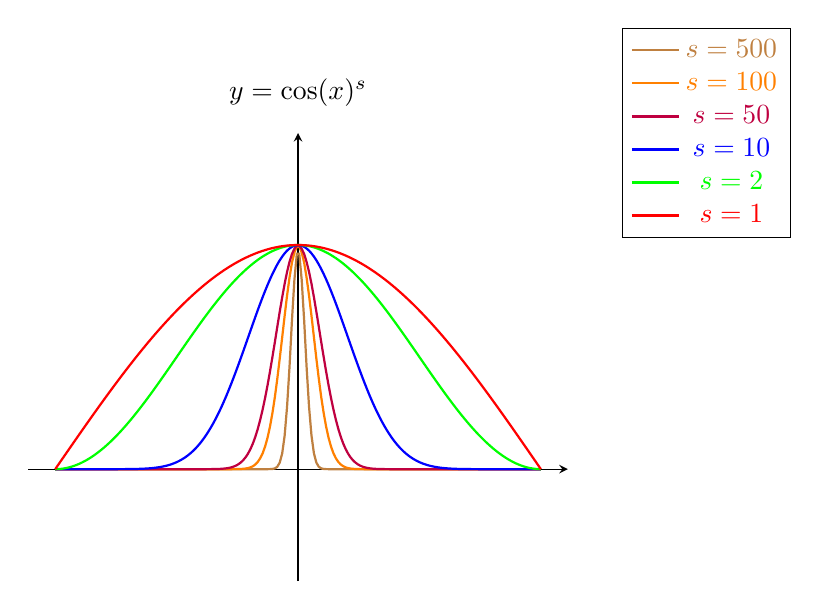
\begin{tikzpicture}
	\begin{axis}[
		xtick=\empty,
		ytick=\empty,
		xmin=-100,
		xmax=100,
		ymin=-0.5,
		ymax=1.5,
		axis x line=center,
		axis y line=center,
		legend style={at={(1.1,1)},anchor=west, title={$y = \cos(x)^s$}},
	]
	\addlegendentry[brown]{$s=500$};
	\addlegendentry[orange]{$s=100$};
	\addlegendentry[purple]{$s=50$};
	\addlegendentry[blue]{$s=10$};
	\addlegendentry[green]{$s=2$};
	\addlegendentry[red]{$s=1$};
	\addplot[color=brown, thick, samples=200, domain=-90:90] {cos(x)^500};
	\addplot[color=orange, thick, samples=200, domain=-90:90] {cos(x)^100};
	\addplot[color=purple, thick, samples=200, domain=-90:90] {cos(x)^50};
	\addplot[color=blue, thick, samples=200, domain=-90:90] {cos(x)^10};
	\addplot[color=green, thick, samples=200, domain=-90:90] {cos(x)^2};
	\addplot[color=red, thick, samples=200, domain=-90:90] {cos(x)^1};
	\end{axis}
	\end{tikzpicture}
    \caption{Cosinus functies verheven tot verschillende machten $s$.}
    \label{fig:cosini}
\end{figure}

$\ora{L}$ kan ontleden worden in $\ora{L_P}$ en $\ora{L_N}$, waar $\ora{L_N}$ evenwijdig is aan $\ora{N}$ en $\ora{L_N}$ loodrecht staat op $\ora{N}$.

\begin{figure}[H]
    \centering
    \includegraphics[width=0.50\textwidth]{L_decomposition.png}
    \caption{$\protect\overrightarrow{L}$ ontleden in componenten $\protect\overrightarrow{L_P}$ en $\protect\overrightarrow{L_N}$}
    \label{fig:L_decomposition}
\end{figure}

Omdat $\left|\ora{N}\right| = 1$, geldt $\left|\ora{L_N}\right|=\langle\ora{N},\ora{L}\rangle$. $\ora{L_N}$ is evenwijdig met $\ora{N}$ dus $\ora{L_N}=\ora{N}\langle\ora{N},\ora{L}\rangle$.

$\ora{L}=\ora{L_P}+\ora{L_N}$ dus $\ora{L_P}=\ora{L}-\ora{L_N}=\ora{L}-\ora{N}\langle\ora{N},\ora{L}\rangle$.

\begin{figure}[H]
    \centering
    \includegraphics[width=0.50\textwidth]{LR_Calculation.png}
    \caption{Het berekenen van $\protect\ora{L_R}$}
    \label{fig:LR_Calculation}
\end{figure}

$\ora{R}$ is aan de andere kant van $\ora{N}$ en heeft dezelfde hoogte als $\ora{R}$ dus $\ora{R}=\ora{L_N}-\ora{L_P}$

Als hierin de eerder verkregen formules gesubstitueerd worden volgt:

\[\ora{R}=\ora{N}\langle\ora{N},\ora{L}\rangle-\ora{L}+\ora{N}\langle\ora{N},\ora{L}\rangle\]
\[\ora{R}=2\ora{N}\langle\ora{N},\ora{L}\rangle-\ora{L}\]

Verder geldt:
\[\cos\left(\angle\left(\ora{R}, \ora{V}\right)\right)=\frac{\langle\ora{R},\ora{V}\rangle}{\left|\ora{R}\right|\left|\ora{V}\right|}\]

Hieruit volgt de volgende formule voor speculaire reflecties:
\[I_S=I_L\left(\frac{\langle\ora{R},\ora{V}\rangle}{\left|\ora{R}\right|\left|\ora{V}\right|}\right)^s\]

Dit kan samengevoegd worden met de eerder vergaarde formule voor diffusie voor een volledige belichtingsformule:

\[
I_P=
I_A+
\sum_{i=l}^{n}I_i\cdot\left[
\frac{\langle \overrightarrow{N}, \overrightarrow{L_i} \rangle}{|\overrightarrow{N}||\overrightarrow{L_i}|}+
\left(\frac{\langle\ora{R_i},\ora{V}\rangle}{\left|\ora{R_i}\right|\left|\ora{V}\right|}\right)^s\right]
\]

In de code ziet de ComputeLighting() functie er nu als volgt uit:

\begin{lstlisting}[language=C++]
double ComputeLighting(Vector3 P, Vector3 N, Vector3 V, double s, Scene scene) {
    double i = 0.0;
    Vector3 L;

    for (Light light: scene.lights) {
        if (light.type == 0) {
            i += light.intensity;
        } else {
            if (light.type == 1) {
                L = subtract(light.position, P);
            } else if (light.type == 2) {
                L = light.direction;
            }

            // Diffuse
            double n_dot_l = dot(N, L);
            if (n_dot_l > 0) {
                i += light.intensity * n_dot_l/magnitude(L);
            }

            // Specular
            if (s != -1) {
                Vector3 R = subtract(multiply(N, 2* dot(N, L)), L);
                double r_dot_v = dot(R, V);
                if (r_dot_v > 0) {
                    i += light.intensity * pow(r_dot_v/(magnitude(R)*magnitude(V)), s);
                }
            }
        }
    }
    return i;
}
\end{lstlisting}

Een object heeft geen speculaire reflecties als $s=-1$. 

Aan de ObjectMaterial() klasse wordt de specular eigenschap toegevoegd:

\begin{lstlisting}[language=C++]
class ObjectMaterial {
    public: 
        Color color;
        double specular;

        ObjectMaterial(Color color, double specular);
        ObjectMaterial();
};
\end{lstlisting}

Nu worden de bollen gerenderd met speculaire reflecties.

\begin{figure}[H]
    \centering
    \includegraphics[width=0.50\textwidth]{renders/specular.png}
    \caption{De bollen gerenderd met speculaire reflecties. De rode bol heeft een hogere waarde $s$ dan de groene bol.}
    \label{fig:specular}
\end{figure}

\subsubsection{Schaduwen}
Om te weten waar schaduwen getekend moeten worden wordt een nieuwe straal vanaf een punt op de vorm afgevuurd richting de camera. Als er een andere vorm tussenzit wordt voor dat punt niet de diffuse en speculaire reflectie berekend. Hiervoor kan de eerder geschreven ClosestIntersection() functie hergebruikt worden. De ComputeLighting functie ziet er dan als volgt uit:

\begin{lstlisting}[language=C++]
double ComputeLighting(Vector3 P, Vector3 N, Vector3 V, double s, Scene scene) {
    double i = 0.0;
    Vector3 L;

    for (Light light: scene.lights) {
        if (light.type == 0) {
            i += light.intensity;
        } else {
            if (light.type == 1) {
                L = subtract(light.position, P);
            } else if (light.type == 2) {
                L = light.direction;
            }

            // Shadow Check
            double shadow_t = ClosestIntersection(P, L, 0.001, 1E9, scene).second;
            if (shadow_t != 1E9) {
                continue;
            } 

            // Diffuse
            double n_dot_l = dot(N, L);
            if (n_dot_l > 0) {
                i += light.intensity * n_dot_l/magnitude(L);
            }

            // Specular
            if (s != -1) {
                Vector3 R = subtract(multiply(N, 2* dot(N, L)), L);
                double r_dot_v = dot(R, V);
                if (r_dot_v > 0) {
                    i += light.intensity * pow(r_dot_v/(magnitude(R)*magnitude(V)), s);
                }
            }
        }
    }
    return i;
}
\end{lstlisting}

Dit zijn alle aanpassingen die gemaakt moeten worden aan de code.

\begin{figure}[H]
    \centering
    \includegraphics[width=0.50\textwidth]{renders/schaduw.png}
    \caption{De bollen gerenderd met schaduwen.}
    \label{fig:schaduw}
\end{figure}

\subsubsection{Reflecties}

Om reflecties te tekenen moet de TraceRay() functie vanaf het raakpunt opnieuw uitgevoerd worden in de tegenovergestelde richting van de normaal. De formule voor reflectie was eerder vastgesteld als:
\[\ora{L}=2\ora{N}\langle\ora{N},\ora{R}\rangle-\ora{R}\]

Daaruit is de volgende functie geschreven:

\begin{lstlisting}[language=C++]
Vector3 ReflectRay(Vector3 R, Vector3 N) {
    return subtract(multiply(N, 2 * dot(N, R)), R);
}
\end{lstlisting}

De TraceRay() functie wordt recursief toegepast:
\begin{lstlisting}[language=C++]
Color TraceRay(Vector3 O, Vector3 D, double t_min, double t_max, Scene scene, int recursion_depth) {   
    std::pair<Sphere, double> closest_intersection = ClosestIntersection(O, D, t_min, t_max, scene);
    Sphere closest_sphere = closest_intersection.first;
    double closest_t = closest_intersection.second;

    if (closest_t==1E9) {
        return RAYWHITE;
    }

    Vector3 P = add(O, multiply(D, closest_t));
    Vector3 N = subtract(P, closest_sphere.center);
    N = multiply(N, 1/magnitude(N));
    Color local_color = multiply(closest_sphere.material.color, ComputeLighting(P, N, multiply(D, -1), closest_sphere.material.specular, scene));

    double r = closest_sphere.material.reflective;
    if (recursion_depth <=0 || r <= 0) {
        return local_color;
    }

    Vector3 R = ReflectRay(multiply(D, -1), N);
    Color reflected_color = TraceRay(P, R, 0.001, 1E9, scene, recursion_depth - 1);

    return add(multiply(local_color, 1 - r), multiply(reflected_color, r)); 

}
\end{lstlisting}

Aan de ObjectMaterial() klasse is de laatste nieuwe eigenschap reflective toegevoegd, de reflectie wordt met deze waarde vermenigvuldigd:

\begin{lstlisting}[language=C++]
class ObjectMaterial {
    public: 
        Color color;
        double specular;
        double reflective;

        ObjectMaterial(Color color, double specular, double reflective);
        ObjectMaterial();
};
\end{lstlisting}

Als reflective lager is dan 0 zijn er geen reflecties voor dat object. Deze kleine toevoegingen maken de basis van de raytracer af.

\begin{figure}[H]
    \centering
    \includegraphics[width=0.50\textwidth]{renders/reflection.png}
    \caption{De bollen gerenderd met reflecties.}
    \label{fig:reflection}
\end{figure}

\subsubsection{Raymarching}

De IntersectRaySphere() functie wordt vervangen door MarchRay(). Verder is het Sphere() object nu weg. In plaats daarvan is er een SDFObject(), die een methode SDF() heeft.

\begin{lstlisting}[language=C++]
double marchRay(Vector3 O, Vector3 D, SDFObject *object, double max_distance, int max_marching_steps, double max_depth) {
    double depth = magnitude(D);

    for (int i = 0; i < max_marching_steps; i++) {
        double distance = object->SDF(add(O, multiply(D, depth)));
        if (distance < max_distance) {
            return depth;
        }

        depth += distance;


        if (depth >= max_depth) {
            return 1E9;
        }
    }

    return 1E9;
}
\end{lstlisting}

Er wordt steeds een stap in de richting van de straal gezet met de grootte van de afstand tot het object, totdat de afstand lager is dan een bepaalde aangegeven grenswaarde.

Verder moet de normaal nog berekend worden. De normaal is gelijk aan de gradiënt van het oppervlakte:

\[\ora{N} = \nabla f(p)\]

Waar $f(p)$ de SDF is.

De definitie van de gradiënt zegt:

\[\nabla f(p)=\left\{\frac{df(p)}{dx},\frac{df(p)}{dy},\frac{df(p)}{dz}\right\}\]

De afgeleide is te benaderen met:

\[\frac{df(p)}{dx}\approx\frac{f\left(p+\begin{pmatrix} \epsilon \\ 0 \\ 0 \end{pmatrix}\right)-f\left(p-\begin{pmatrix} \epsilon \\ 0 \\ 0 \end{pmatrix}\right)}{2\epsilon}\]

Bij de afgeleide geldt $\lim\limits_{\epsilon \to 0}$ dus bij de de numerieke benadering is $\epsilon$ een heel klein getal.

Hieruit volgt:

\[
\ora{N}=\begin{pmatrix} 
f\left(p+\begin{pmatrix} \epsilon \\ 0 \\ 0 \end{pmatrix}\right)-f\left(p-\begin{pmatrix} \epsilon \\ 0 \\ 0 \end{pmatrix}\right) \\
f\left(p+\begin{pmatrix} 0 \\ \epsilon \\ 0 \end{pmatrix}\right)-f\left(p-\begin{pmatrix} 0 \\ \epsilon \\ 0 \end{pmatrix}\right) \\
f\left(p+\begin{pmatrix} 0 \\ 0 \\ \epsilon \end{pmatrix}\right)-f\left(p-\begin{pmatrix} 0 \\ 0 \\ \epsilon \end{pmatrix}\right)
\end{pmatrix}\]

In de code ziet dat er als volgt uit:
\begin{lstlisting}[language=C++]
Vector3 estimateNormal(SDFObject *object, Vector3 P) {
    return normalize((Vector3){
        object->SDF((Vector3){P.x + EPSILON, P.y, P.z}) - object->SDF((Vector3){P.x - EPSILON, P.y, P.z}),
        object->SDF((Vector3){P.x, P.y + EPSILON, P.z}) - object->SDF((Vector3){P.x, P.y - EPSILON, P.z}),
        object->SDF((Vector3){P.x, P.y, P.z  + EPSILON}) - object->SDF((Vector3){P.x, P.y, P.z - EPSILON})
    });
}
\end{lstlisting}

In plaats van een vector van de bollen in het Scene() object is er nu een vector van pointers naar de verschillende SDFObjects. De bol wordt nu als volgt gedefiniëerd:
\begin{lstlisting}[language=C++]
class SDFSphere: public SDFObject {
    public:
        double radius;

        SDFSphere(Vector3 center, double radius, ObjectMaterial material);
        SDFSphere();

        virtual double SDF(Vector3 P);
};
\end{lstlisting}

Met als SDF:

\begin{lstlisting}[language=C++]
double SDFSphere::SDF(Vector3 P) {
    return magnitude(subtract(P, center)) - radius;
}
\end{lstlisting}

Verder is de initialisatie van de scène verplaatst naar de functie initScene(). Als volgt wordt hiermee een scène gedefinieerd:
\begin{lstlisting}[language=C++]
void initScene(Scene *scene) {
    scene -> AddObject(new SDFSphere(
        (Vector3){-1.7, 0, 5}, // center
        0.6, //radius
        ObjectMaterial (
            (Color){255, 0, 0, 255}, // color
            500, // specular
            0.1 // reflective
        )
    ));

    scene -> AddObject(new SDFSphere(
        (Vector3){0, 0, 5}, // center
        1, //radius
        ObjectMaterial (
            (Color){0, 255, 0, 255}, // color
            100, // specular
            0.1 // reflective
        )
    ));

    scene -> AddObject(new SDFSphere(
        (Vector3){1.7, 0, 5}, // center
        0.6, //radius
        ObjectMaterial (
            (Color){0, 0, 255, 255}, // color
            500, // specular
            0.1 // reflective
        )
    ));

    scene -> AddLight(Light(
        0, // Ambient
        0.2
    ));

    scene -> AddLight(Light(
        1, // Point
        0.6,
        (Vector3){2, 1, 0}
    ));

    scene -> AddLight(Light(
        2, // Directional
        0.2,
        (Vector3){1, 4, 4}
    ));
}
\end{lstlisting}

Daaruit volgt de eerste render die gebruik maakt van raymarching.

\begin{figure}[H]
    \centering
    \includegraphics[width=0.50\textwidth]{renders/first_raymarched.png}
    \caption{De bollen, nu gedefiniëerd met SDFs.}
    \label{fig:first_raymarched}
\end{figure}

\clearpage

\subsubsection{SDFs}

\paragraph{Balk}
Voor de balk is de volgende SDF gedefiniëerd:
\begin{lstlisting}[language=C++]
double SDFBox::SDF(Vector3 P) {
    P = subtract(P, center);
    Vector3 b = box;
    Vector3 q = subtract(abs(P), b);
    return magnitude(max(q,0.0)) + std::min((double)std::max(q.x,std::max(q.y,q.z)),0.0);
}
\end{lstlisting}
Waarin \emph{box} de lengte, breedte en hoogte van de balk beschrijft.

\begin{figure}[H]
    \centering
    \includegraphics[width=0.50\textwidth]{renders/boxes.png}
    \caption{Verschillende balken gerenderd met een SDF.}
    \label{fig:boxes}
\end{figure}

\clearpage

\paragraph{Torus}
Voor de torus is de volgende functie gedefiniëerd:
\begin{lstlisting}[language=C++]
double SDFTorus::SDF(Vector3 P) {
    P = subtract(P, center);
    Vector2 q = (Vector2){magnitude((Vector2){P.x,P.z})-holes.x,P.y};
    return magnitude(q)-holes.y;
}
\end{lstlisting}

Waarin $holes$ een Vector2 is met de straal van de torus, en de dikte.

\begin{figure}[H]
    \centering
    \includegraphics[width=0.50\textwidth]{renders/tori.png}
    \caption{Verschillende torussen gerenderd met een SDF.}
    \label{fig:tori}
\end{figure}

\paragraph{Vlak}
Voor het vlak is de volgende functie gedefiniëerd:
\begin{lstlisting}[language=C++]
double SDFPlane::SDF(Vector3 P) {
    return abs(P.y - center.y);
}
\end{lstlisting}



\begin{figure}[H]
    \centering
    \includegraphics[width=0.50\textwidth]{renders/plane.png}
    \caption{Een vlak gerenderd met een SDF.}
    \label{fig:plane}
\end{figure}

\paragraph{Cylinder}
Voor de cylinder is de volgende functie gedefiniëerd:
\begin{lstlisting}[language=C++]
double SDFCylinder::SDF(Vector3 P) {
    P = subtract(P, center);
    Vector2 d = (Vector2){
        abs(magnitude((Vector2){P.x, P.z}))-radius,
        abs(P.y) - height
    };
    return std::min((double)std::max(d.x, d.y), 0.0) + magnitude(max(d, 0.0));
}
\end{lstlisting}


\begin{figure}[H]
    \centering
    \includegraphics[width=0.50\textwidth]{renders/cylinders.png}
    \caption{Cylinders gerenderd met SDFs.}
    \label{fig:cylinders}
\end{figure}


\subsubsection{SDF operaties}

De boolean operaties \emph{union}, \emph{subtraction} en \emph{intersection} worden ook als SDFObject() toegevoegd. Met de desbetreffende vormen als argumenten die ook van type SDFObject() zijn.

Het SDFUnion() object is bijvoorbeeld als volgt gedefiniëerd:

\begin{lstlisting}[language=C++]
class SDFUnion: public SDFObject {
    public:
        Vector3 center;
        
        SDFObject *first_object;
        SDFObject *second_object;

        SDFUnion(Vector3 center, SDFObject *first_object, SDFObject *second_object, ObjectMaterial material);
        SDFUnion();

        virtual double SDF(Vector3 P);
};
\end{lstlisting}

Met als SDF:

\begin{lstlisting}[language=C++]
double SDFUnion::SDF(Vector3 P) {
    P = subtract(P, center);
    return std::min(first_object -> SDF(P), second_object -> SDF(P));
}
\end{lstlisting}


\begin{figure}[H]
    \centering
    \includegraphics[width=0.50\textwidth]{renders/union.png}
    \caption{De \emph{union} tussen een bol en een torus.}
    \label{fig:union}
\end{figure}

De SDF van \emph{subtraction} is als volgt:

\begin{lstlisting}[language=C++]
double SDFSubtraction::SDF(Vector3 P) {
    P = subtract(P, center);
    return std::max(first_object -> SDF(P), -1 * second_object -> SDF(P));
}
\end{lstlisting}


\begin{figure}[H]
    \centering
    \includegraphics[width=0.50\textwidth]{renders/subtraction.png}
    \caption{De \emph{subtraction} tussen twee bollen.}
    \label{fig:subtraction}
\end{figure}

De SDF van \emph{intersection} is als volgt:

\begin{lstlisting}[language=C++]
double SDFIntersection::SDF(Vector3 P) {
    P = subtract(P, center);
    return std::max(first_object -> SDF(P), second_object -> SDF(P));
}
\end{lstlisting}


\begin{figure}[H]
    \centering
    \includegraphics[width=0.50\textwidth]{renders/intersection.png}
    \caption{De \emph{intersection} tussen twee bollen.}
    \label{fig:intersection}
\end{figure}
\subsubsection{Transformaties}

De volgende rotatiematrices beschrijven hoe een coördinaat respectievelijk rondom de x-, y-, en z-as gedraaid worden met hoek $\theta$.
\[
R_x(\theta) = \begin{bmatrix}
1 &  0            &  0           \\
0 &  \cos \theta  & -\sin \theta \\
0 &  \sin \theta & \cos \theta \\
\end{bmatrix}
\]
\[
R_y(\theta) = \begin{bmatrix}
\cos \theta & 0 & \sin \theta \\
0           & 1 &  0           \\
-\sin \theta & 0 &  \cos \theta \\
\end{bmatrix}
\]
\[
R_z(\theta) = \begin{bmatrix}
\cos \theta & -\sin \theta & 0 \\
\sin \theta &  \cos \theta & 0 \\
0           &  0           & 1 \\
\end{bmatrix}
\]
Vermenigvuldigd met $\{x,y,z\}$ geeft dat:
\[
R_x(\theta)\times
\begin{bmatrix} x \\ y \\ z \\ \end{bmatrix}=
\begin{bmatrix}
x \\
y \cos \theta - z \sin \theta \\
y \sin \theta + z \cos \theta \\
\end{bmatrix} 
\]
\[
R_y(\theta)\times
\begin{bmatrix} x \\ y \\ z \\ \end{bmatrix}=
\begin{bmatrix}
x \cos \theta + z \sin \theta \\
y \\
-x \sin \theta + z \cos \theta \\
\end{bmatrix} 
\]
\[
R_z(\theta) \times
\begin{bmatrix} x \\ y \\ z \\ \end{bmatrix}=
\begin{bmatrix}
x \cos \theta - y \sin \theta \\
x \sin \theta + y \cos \theta \\
z \\
\end{bmatrix} 
\]

In de code is er een SDFRotate() object. Standaard zullen de rotaties in de volgorde XYZ uitgevoerd worden. Met de volgende SDF:
\begin{lstlisting}[language=C++]
double SDFRotate::SDF(Vector3 P) {
    P = subtract(P, center);

    P = (Vector3){
        P.x,
        P.y * cosx - P.z * sinx,
        P.y * sinx + P.z * cosx,
    }; // X rotation
    P = (Vector3){
        P.x * cosy + P.z * siny,
        P.y,
        - P.x * siny + P.z * cosy,
    }; // Y rotation
    P = (Vector3){
        P.x * cosz - P.y * sinz,
        P.x * sinz + P.y * cosz,
        P.z,
    }; // Z rotation
    return object -> SDF(P);
}
\end{lstlisting}

De verschillende cosinus en sinus berekeningen worden bij initialisatie berekend.

\begin{lstlisting}[language=C++]
void SDFRotate::initializeTransformations() {
    double x_rad = radian(x_angle);
    double y_rad = radian(y_angle);
    double z_rad = radian(z_angle);

    cosx = cos(radian(x_angle));
    sinx = sin(radian(x_angle));

    cosy = cos(radian(y_angle));
    siny = sin(radian(y_angle));

    cosz = cos(radian(z_angle));
    sinz = sin(radian(z_angle));
}
\end{lstlisting}

De volgende testscène laat de werking van rotaties zien:

\begin{figure}[H]
    \centering
    \includegraphics[width=0.50\textwidth]{renders/rotaties.png}
    \caption{Verschillende rotaties.}
    \label{fig:rotaties}
\end{figure}
\subsubsection{Driehoeken}
Een driehoek is gedefinieerd door drie hoekpunten. Die drie punten liggen op een vlak. Om de normaal van dat vlak te krijgen nemen we het kruisproduct van twee niet-paralelle vectoren op dat vlak. 

\begin{figure}[H]
	\centering
	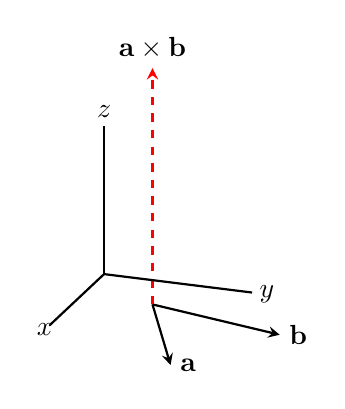
\begin{tikzpicture}[scale=1,    vector/.style={-stealth, thick},    origin/.style={black, fill=white, inner sep=1.5pt}]
		% draw the vectors
		\draw[vector] (1,0,1) -- (2,0,3);
		\draw[vector] (1,0,1) -- (3,0,2);
		\draw[vector,red,dashed] (1,0,1) -- (1,3,1);
		% add labels
		\node[right] at (2,0,3) {$\mathbf{a}$};
		\node[right] at (3,0,2) {$\mathbf{b}$};
		\node[above] at (1,3,1) {$\mathbf{a} \times \mathbf{b}$};
		% set the view
		\tdplotsetmaincoords{70}{110}
		\begin{scope}[tdplot_main_coords]
			% draw the coordinate system
			\draw[thick] (0,0,0) -- (2,0,0) node[pos=1.1]{$x$};
			\draw[thick] (0,0,0) -- (0,2,0) node[pos=1.1]{$y$};
			\draw[thick] (0,0,0) -- (0,0,2) node[pos=1.1]{$z$};
		\end{scope}3
	\end{tikzpicture}
	\caption{Het kruisproduct van $a$ en $b$.}
	\label{fig:kruisproduct}
\end{figure}

Zoals eerder genoemd wordt de straal beschreven als een parameter-lijn in de vorm:

\[l:P=O+t\ora{D}\]

Met de vergelijking van een vlak

\[v:ax+by+cz=d\]

Waarbij:

\[\ora{n}=\begin{pmatrix} a \\ b \\ c \\ \end{pmatrix}\]

Als we een driehoek nemen met punten $P$, $Q$ en $R$ geldt:

\[\ora{n}=\ora{PQ}\times\ora{PR}\]

Om $d$ te krijgen nemen moet slechts enig punt op de driehoek ingevuld worden in de vergelijking van het vlak.

Voor het snijpunt van de lijn en het vlak moet punt P van de lijn ingevuld worden in de vergelijking van het vlak. Daaruit volgt:

\[t=\frac{d-aO_x-bO_y-cO_z}{a\ora{D_x}+b\ora{D_y}+c\ora{D_z}}\]

Hiermee kan een vlak getekend worden, om een driehoek te tekenen moet nog gecheckt worden of het punt binnen het vlak in die driehoek ligt.

Bij een driehoek $ABC$ met punt $P$ wordt de som van de oppervlakten van driehoeken $ABP$, $ACP$ en $BCP$ vergeleken met het oppervlakte van $ABC$. Als het punt in de driehoek ligt zijn die gelijk, anders is de som groter.
\begin{figure}[H]
	\centering
	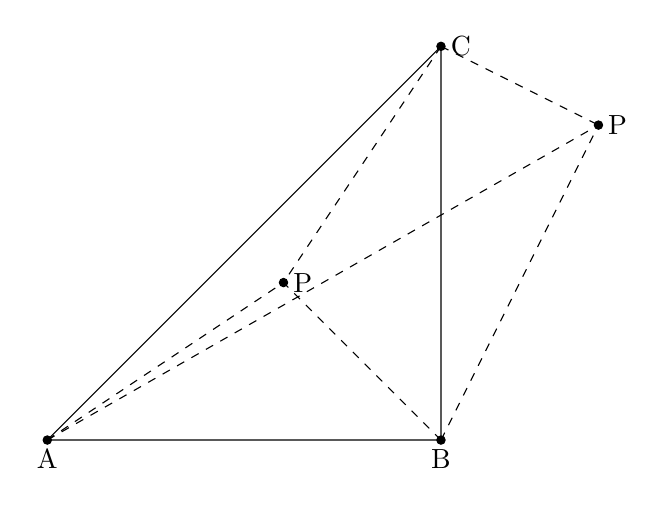
\begin{tikzpicture}[]
		\coordinate (A) at (0,0);
		\coordinate (B) at (5,0);
		\coordinate (C) at (5,5);
		
		\coordinate (P) at (3,2);
		\coordinate (P2) at (7,4);
		
		\node[below] at (A) {A};
		\node[below] at (B) {B};
		\node[right] at (C) {C};
		
		\filldraw (A) circle (1.5pt);
		\filldraw (B) circle (1.5pt);
		\filldraw (C) circle (1.5pt);
		
		\filldraw (P) circle (1.5pt);
		
		\node[right] at (P) {P};
		
		\filldraw (P2) circle (1.5pt);
		
		\node[right] at (P2) {P};
		
		\draw (A) -- (B) -- (C) -- (A);
		
		\draw[dashed] (A) -- (P);
		\draw[dashed] (B) -- (P);
		\draw[dashed] (C) -- (P);
		
		\draw[dashed] (A) -- (P2);
		\draw[dashed] (B) -- (P2);
		\draw[dashed] (C) -- (P2);
	\end{tikzpicture}
	\caption{De som van de driehoeken die $P$ buiten de driehoek vormt met de hoekpunten is groter dan de som van $P$ binnen de driehoek.}
	\label{fig:driehoek_punt_check}
\end{figure}

Om het oppervlakte te berekenen wordt gebruik gemaakt van Herons formule:

\[T=\sqrt{s(s-a)(s-b)(s-c)}\]

Waarbij $a$, $b$ en $c$ zijden van de driehoek zijn en $s=\frac{1}{2}(a+b+c)$.

Dit is als volgt in code beschreven:

\begin{lstlisting}[language=c++]
double triangleArea(Vector3 p1, Vector3 p2, Vector3 p3) {
	double a = magnitude(subtract(p1, p2));
	double b = magnitude(subtract(p2, p3));
	double c = magnitude(subtract(p3, p1));
	double s = 0.5 * (a + b + c);
	
	return sqrt(s*(s-a)*(s-b)*(s-c));
}

bool pointInTriangle(Vector3 P, Vector3 A, Vector3 B, Vector3 C) {
	return triangleArea(A, B, C) + EPSILON >= triangleArea(P, A, B) + triangleArea(P, A, C) + triangleArea(P, B, C);
}

bool isBackface(Vector3 corner, Vector3 O, Vector3 N) {
	return dot(subtract(corner, O), N) >= 0;
}

double intersectRayTriangle(Vector3 O, Vector3 D, MeshObject* mesh, int faceIndex) {
	Vector3 n = mesh -> FaceNormal(faceIndex);
	
	Vector3 v1 = mesh -> vertices[mesh -> faces[faceIndex].cornerIndices[0]].pos;
	Vector3 v2 = mesh -> vertices[mesh -> faces[faceIndex].cornerIndices[1]].pos;
	Vector3 v3 = mesh -> vertices[mesh -> faces[faceIndex].cornerIndices[2]].pos;
	
	double d = n.x * v1.x + n.y * v1.y + n.z * v1.z;
	double t = (d-n.x*O.x-n.y*O.y-n.z*O.z)/(n.x*D.x+n.y*D.y+n.z*D.z);
	
	Vector3 P = add(O, multiply(D, t));
	
	if (!pointInTriangle(P, v1, v2, v3) | isBackface(v1, O, mesh -> FaceNormal(faceIndex))) {
		return 1E9;
	}
	return t;
}
\end{lstlisting}

\subsubsection{Mesh Representatie}
Voor mesh representatie worden de in de inleiding genoemde \textit{face-vertex meshes} gebruikt. 

De mesh staat in de code als volgt:
\begin{lstlisting}[language=c++]
class MeshObject {
	public:
	ObjectMaterial material;
	
	std::vector<Face> faces;
	std::vector<Vertex> vertices;
	
	int AddVertex(Vector3 P);
	int AddFace(int v1, int v2, int v3);
	
	Vector3 FaceNormal(int f);
	
	MeshObject(ObjectMaterial material);
	MeshObject();
};
\end{lstlisting}

Daar wordt gebruikt gemaakt van de types Face en Vertex, die als volgt zijn gedefiniëerd. Met referenties naar de index van de bijbehorende zijden/punten in de arrays zoals gedefinieerd in MeshObject. Verder is voor elke zijde de normaal van te voren berekend, om latere berekeningen te verminderen.

\begin{lstlisting}[language=c++]
struct Vertex {
	Vector3 pos;
	std::vector<int> faceIndices;
};

struct Face {
	int cornerIndices[3];
	Vector3 normal;
};
\end{lstlisting}

\begin{lstlisting}[language=c++]
int MeshObject::AddVertex(Vector3 P) {
	Vertex V = {P, {}};
	vertices.push_back(V);
	return vertices.size()-1;
}

int MeshObject::AddFace(int p1, int p2, int p3) {
	Vector3 P1 = vertices[p1].pos;
	Vector3 P2 = vertices[p2].pos;
	Vector3 P3 = vertices[p3].pos;
	
	Face F = {{p1, p2, p3}, normalize(cross(subtract(P1, P2), subtract(P1, P3)))};
	faces.push_back(F);
	int faceIndex = faces.size()-1;
	vertices[p1].faceIndices.push_back(faceIndex);
	vertices[p2].faceIndices.push_back(faceIndex);
	vertices[p3].faceIndices.push_back(faceIndex);
	return faceIndex;
}
\end{lstlisting}

\subsubsection{Polygonale primitieven}

Voor de balk worden zowel de hoekpunten als de zijden handmatig gedefinieerd.

\begin{lstlisting}[language=c++]
void generateBox(MeshObject* mesh, Vector3 center, Vector3 box) {
	Vector3 base = subtract(center, multiply(box, 0.5));
	
	int p000 = mesh -> AddVertex(base);
	int p001 = mesh -> AddVertex(add(base, {0, 0, box.z}));
	int p010 = mesh -> AddVertex(add(base, {0, box.y, 0}));
	int p011 = mesh -> AddVertex(add(base, {0, box.y, box.z}));
	int p100 = mesh -> AddVertex(add(base, {box.x, 0, 0}));
	int p101 = mesh -> AddVertex(add(base, {box.x, 0, box.z}));
	int p110 = mesh -> AddVertex(add(base, {box.x, box.y, 0}));
	int p111 = mesh -> AddVertex(add(base, box));
	
	mesh -> AddFace(p000, p010, p100); // FRONT
	mesh -> AddFace(p110, p100, p010); // FRONT
	mesh -> AddFace(p010, p011, p110); // TOP
	mesh -> AddFace(p110, p011, p111); // TOP
	mesh -> AddFace(p100, p110, p111); // RIGHT
	mesh -> AddFace(p100, p111, p101); // RIGHT
	mesh -> AddFace(p000, p100, p001); // BOTTOM
	mesh -> AddFace(p100, p101, p001); // BOTTOM
	mesh -> AddFace(p001, p101, p011); // BACK
	mesh -> AddFace(p111, p011, p101); // BACK
	mesh -> AddFace(p000, p011, p010); // LEFT
	mesh -> AddFace(p000, p001, p011); // LEFT
}
\end{lstlisting}

Voor de bol wordt de zogenoemde \textit{UV-sphere} gebruikt. % Bron voor UV-sphere?
Daarbij wordt de bol opgedeeld in verticaal verdeelde ringen, die vervolgens een bepaalde resolutie hebben. Dan worden de \textit{quads} tussen de ringen ingevuld.

\begin{lstlisting}[language=c++]
void generateSphere(MeshObject* mesh, Vector3 center, double radius, int rings, int detail) {
	int pTop = mesh -> AddVertex(add(center, {0, radius, 0}));
	int pBottom = mesh -> AddVertex(subtract(center, {0, radius, 0}));
	
	int currentVertex;
	
	for (int ring = 1; ring <= detail; ring ++) {
		double ringHeight = center.y + radius - ring*radius*2/rings;
		double currentRadius = sqrt(1-pow((1-(double)ring/rings)*2-1, 2))*radius;
		std::cout << currentRadius << std::endl;
		for (int i = 0; i < detail; i++) {
			currentVertex = mesh -> AddVertex({
				center.x+currentRadius*sin(2*M_PI*i/detail),
				ringHeight,
				center.z+currentRadius*cos(2*M_PI*i/detail)
			});
			if (ring == 1) {
				mesh -> AddFace(pTop, currentVertex - 1, currentVertex);
			} else if (i != 0) {
				mesh -> AddFace(currentVertex - detail, currentVertex - 1, currentVertex);
				mesh -> AddFace(currentVertex - detail, currentVertex - detail - 1, currentVertex - 1);
				if (ring == detail) {
					mesh -> AddFace(pBottom, currentVertex - 1, currentVertex);
				}
			}
		}
	}
}
\end{lstlisting}

Voor de cylinder worden twee cirkels aan punten aan de boven- en onderkant aangemaakt. Die cirkels worden met het \textit{ear clipping}\footnote{bron} algoritme ingevuld. Daarna worden de twee cirkels met elkaar verbonden met quads.

\begin{lstlisting}[language=c++]
void generateCylinder(MeshObject* mesh, Vector3 center, double height, double radius, int detail) {
	int lastVertex = mesh -> vertices.size()-1;
	int currentVertex;
	
	for (int i = 0; i < detail; i++) { // TOP RING
		currentVertex = mesh -> AddVertex({
			center.x+radius*sin(2*M_PI*i/detail), 
			center.y+0.5*height, 
			center.z+radius*cos(2*M_PI*i/detail)
		});
		if (i > 1) {
			mesh -> AddFace(lastVertex+1, currentVertex - 1, currentVertex);
		}
	} 
	for (int i = 0; i < detail; i++) { // BOTTOM RING
		currentVertex = mesh -> AddVertex({
			center.x+radius*sin(2*M_PI*i/detail), 
			center.y-0.5*height, 
			center.z+radius*cos(2*M_PI*i/detail)
		});
		if (i != 0) {
			mesh -> AddFace(currentVertex, currentVertex - detail - 1, currentVertex - 1);
			mesh -> AddFace(currentVertex, currentVertex - detail, currentVertex - detail - 1);
			if (i != 1) {
				mesh -> AddFace(lastVertex+1+detail, currentVertex, currentVertex - 1);
			}
		}
	}
}
\end{lstlisting}

\subsubsection{Meten}
\begin{lstlisting}[language=c++]
auto start = std::chrono::high_resolution_clock::now();
int x = -canvas.width/2;

while (!WindowShouldClose()) {
	BeginDrawing();

	for (int y = -canvas.height/2; y < canvas.height/2; y++) {
		Vector3 D = normalize(vp.CanvasToViewport(canvas, x, y));
		Color color = TraceRay(O, D, 1, 1E9, scene, 5);
		canvas.PutPixel(x, y, color);
	}
	
	if (x >= canvas.width/2) {
		auto stop = std::chrono::high_resolution_clock::now();
		auto duration = std::chrono::duration_cast<std::chrono::milliseconds>(stop - start);
		std::cout << duration.count() << " milliseconds" << std::endl;
		x = -canvas.width/2;
		start = std::chrono::high_resolution_clock::now();
	}
	
	x++;
	
	EndDrawing();
}
\end{lstlisting}

\clearpage
\section{Methode}
Om de nu ontwikkelde renderprogramma's met elkaar te vergelijken wordt de rendersnelheid per frame gemeten. Voor elke scène wordt dit tien keer gedaan, om eventuele ruis in de data te verminderen. 
\subsection{Testscènes}
Resolutie: $1000\times 1000$
\paragraph{Test \#1: Enkele bol}
$ $
\begin{figure}[H]
	\centering
	\subfloat[Enkele bol als SDF]{
		\includegraphics[width=0.3\textwidth]{renders/test_001_sdf.png}
		\label{fig:test_001_sdf}
	}
	\subfloat[Enkele bol als mesh met 7 cirkels in beide richtingen]{
		\includegraphics[width=0.3\textwidth]{renders/test_001_mesh_lowres.png}
		\label{fig:test_001_mesh_lowres}
	}
	\subfloat[Enkele bol als mesh met 14 cirkels in beide richtingen]{
		\includegraphics[width=0.3\textwidth]{renders/test_001_mesh_highres.png}
		\label{fig:test_001_mesh_highres}
	}
	\caption{Enkele bol}
\end{figure}

\paragraph{Test \#2: Enkele balk}
$ $
\begin{figure}[H]
	\centering
	\subfloat[Enkele balk als SDF]{
		\includegraphics[width=0.3\textwidth]{renders/test_002_sdf.png}
		\label{fig:test_002_sdf}
	}
	\subfloat[Enkele balk als mesh]{
		\includegraphics[width=0.3\textwidth]{renders/test_002_mesh.png}
		\label{fig:test_002_mesh}
	}
\end{figure}
\clearpage
\paragraph{Test \#3: Enkele cylinder}
$ $
\begin{figure}[H]
	\centering
	\subfloat[Enkele cylinder als SDF]{
		\includegraphics[width=0.3\textwidth]{renders/test_003_sdf.png}
		\label{fig:test_003_sdf}
	}
	\subfloat[Enkele cylinder als mesh met een cirkel met 10 punten]{
		\includegraphics[width=0.3\textwidth]{renders/test_003_mesh_lowres.png}
		\label{fig:test_003_mesh_lowres}
	}
	\subfloat[Enkele cylinder als mesh met een cirkel met 50 punten]{
		\includegraphics[width=0.3\textwidth]{renders/test_003_mesh_highres.png}
		\label{fig:test_003_mesh_highres}
	}
	\caption{Enkele cylinder}
\end{figure}
\paragraph{Test \#4: Grote balk met bol erboven}
$ $
\begin{figure}[H]
	\centering
	\subfloat[Grote balk met bol erboven als SDF]{
		\includegraphics[width=0.3\textwidth]{renders/test_004_sdf.png}
		\label{fig:test_004_sdf}
	}
	\subfloat[Grote balk met bol erboven als mesh met 7 cirkels in beide richtingen]{
		\includegraphics[width=0.3\textwidth]{renders/test_004_mesh_lowres.png}
		\label{fig:test_004_mesh_lowres}
	}
	\subfloat[Grote balk met bol erboven als mesh met 14 cirkels in beide richtingen]{
		\includegraphics[width=0.3\textwidth]{renders/test_004_mesh_highres.png}
		\label{fig:test_004_mesh_highres}
	}
	\caption{Grote balk met bol erboven}
\end{figure}
\clearpage
\paragraph{Test \#5: Twee balken tegenover elkaar met bol ertussen}
$ $
\begin{figure}[H]
	\centering
	\subfloat[Twee balken tegenover elkaar met bol ertussen als SDF]{
		\includegraphics[width=0.3\textwidth]{renders/test_005_sdf.png}
		\label{fig:test_005_sdf}
	}
	\subfloat[Twee balken tegenover elkaar met bol ertussen als mesh met 7 cirkels in beide richtingen]{
		\includegraphics[width=0.3\textwidth]{renders/test_005_mesh_lowres.png}
		\label{fig:test_005_mesh_lowres}
	}
	\subfloat[Twee balken tegenover elkaar met bol ertussen als mesh met 14 cirkels in beide richtingen]{
		\includegraphics[width=0.3\textwidth]{renders/test_005_mesh_highres.png}
		\label{fig:test_005_mesh_highres}
	}
	\caption{Twee balken tegenover elkaar met bol ertussen}
\end{figure}

\paragraph{Test \#6: Veel bollen}
$ $
\begin{figure}[H]
\centering
\subfloat[Veel bollen als SDF]{
	\includegraphics[width=0.3\textwidth]{renders/test_006_sdf.png}
	\label{fig:test_006_sdf}
}
\subfloat[Veel bollen als mesh]{
\includegraphics[width=0.3\textwidth]{renders/test_006_mesh_lowres.png}
\label{fig:test_006_mesh_lowres}
}
\caption{Veel bollen}
\end{figure}
\clearpage
\paragraph{Test \#7: Balk, bol en cylinder}
$ $
\begin{figure}[H]
\centering
\subfloat[Balk, bol en cylinder als SDF]{
	\includegraphics[width=0.3\textwidth]{renders/test_007_sdf.png}
	\label{fig:test_007_sdf}
}
\subfloat[Balk, bol en cylinder als mesh met een bol met 7 cirkels in beide richtingen en een cylinder met 10 cirkelpunten]{
	\includegraphics[width=0.3\textwidth]{renders/test_007_mesh_lowres.png}
	\label{fig:test_007_mesh_lowres}
}
\subfloat[Balk, bol en cylinder als mesh met een bol met 14 cirkels in beide richtingen en een cylinder met 50 cirkelpunten]{
	\includegraphics[width=0.3\textwidth]{renders/test_007_mesh_highres.png}
	\label{fig:test_007_mesh_highres}
}
\caption{Balk, bol en cylinder}
\end{figure}
\clearpage
\section{Resultaten}

\begin{table}[H]
\centering
\begin{tabular}{| c | c c c || c c |}
	\hline
	Test & SDF & Mesh (Lowres) & Mesh (Highres) & $\text{lowres}/\text{sdf}$ & $\text{highres}/\text{sdf}$ \\
	\hline
	1 & 17325 & 90676 & 398031 & 5,23 & 22,97 \\
	2 & 16674 & 6820 & - & 0,41 & - \\
	3 & 16750 & 22801 & 123630 & 1,36 & 7,00 \\
	4 & 18481 & 85601 & 335891 & 4,63 & 18,18 \\
	5 & 90870 & 230034 & 790342 & 2,53 & 8,70 \\
	6 & 100984 & 2383653 & - & 23,60 & - \\
	7 & 16721 & 65967 & 275203 & 3,95 & 16,46 \\
	\hline
\end{tabular}
\caption{Verschillende testen samen}
\end{table}

Het wordt snel duidelijk dat het renderen met \textit{signed distance functions} velen malen sneller is dan met polygonen. Naast test 2, met de balk, is het in elke situatie sneller. Bovendien geeft de SDF ook betere kwaliteit renders, aangezien er geen randen tussen driehoeken zichtbaar zijn. In sommige situaties is het zelfs meer dan 23 keer zo snel. De individuele resultaten staan beschreven in Appendix \ref{resultaten}.
\section{Nauwkeurigheidsanalyse}
\begin{table}[H]
	\centering
	\begin{tabular}{| c | c c c |}
		\hline
		Test & SDF & Mesh (Lowres) & Mesh (Highres) \\
		\hline
		1 & 132,7 & 257,8 & 758,0\\
		2 & 16,3 & 39,3 & - \\
		3 & 86,6 & 123,3 & 759,8  \\
		4 & 80,3 & 4146,2 & 12539,8 \\
		5 & 3129,1 & 6251,9 & 17034,1 \\
		6 & 1623,9 & 34417,9 & - \\
		7 & 79,8 & 1595,3 & 4226,3 \\
		\hline
	\end{tabular}
	\caption{Standaarddeviaties}
\end{table}
De standaarddeviaties lopen in sommige situaties op tot wel 34 seconden, echter is het verschil tussen de mesh- en sdf-resultaten in iedere situatie meerdere standaarddeviaties groot. Dit betekent dat de resultaten als significant beschouwd kunnen worden. 

\section{Conclusie}
Het blijkt uit de resultaten duidelijk dat het renderen met SDF's significant sneller is dan met meshes in alles behalve de allersimpelste situaties. Bovendien hebben de SDF's een visuele kwaliteit die met meshes bijna niet te evenaren is. 

In de hypothese was gesteld dat de SDF's sneller zouden zijn in de meeste situaties, maar dat meshes simpele objecten sneller zouden kunnen renderen. Uit de resultaten blijkt een nog sterker voordeel. 

Verder zijn er vragen gesteld over het gemak van het maken van scènes met SDF's tegenover meshes. Aangezien er geen editor gemaakt is voor dit onderzoek kan daar geen antwoord op gegeven worden.

\section{Discussie}

Er kunnen wel vragen gesteld worden bij de implementatie van de polygons en meshes. Zo zal er in professionele programma's meer aandacht gestoken zijn in het geheugengebruik van de meshes. Verder wordt er gebruik gemaakt van \textit{bounding boxes} rondom meshes zodat niet elke straal met elke driehoek in de scène vergeleken hoeft te worden.\cite{BoundingVolumeHierarchy} Dit zou bijvoorbeeld scène 6 een enorme snelheidsboost geven. 

Om in de toekomst de render engine verder uit te werken is het verbeteren van de rendersnelheden van het hoogste belang. De beste manier om dit te doen is het gebruik van de gpu. Raytracing is onderdeel van de klasse \textit{embarrassingly parallelizable problems}. Omdat lichtstralen geen massa hebben, hebben ze geen invloed op elkaar. Vanuit dit principe is elke straal te zien als een los programma die apart uitgevoerd kan worden. De GPU is gespecialiseerd in het uitvoeren van die parallelle taken. De raytracer zou geschreven kunnen worden als zogeheten \textit{fragment shader}. Een andere optie is de \textit{compute shader}, die in theorie beter schaalbaar is.

Verder is een duidelijke \textit{user interface} van belang. Eén potentiele optie is een \textit{node based editor}, waarin de SDF's visueel veranderd een aangepast kunnen worden. Dit systeem past goed bij de modulariteit die het huidige ontwikkelde systeem al met zich meebrengt.

\begin{figure}[H]
	\centering
	\includegraphics[width=\textwidth]{node_editor.png}
	\caption{Node Based SDF Editor Markup}
	\label{fig:node_editor}
\end{figure}
\clearpage
\section{Nawoord}
Bedankt aan mijn moeder Arria Gosman.
Bedankt aan Ina, voor haar mentale steun.
\clearpage
\section{Literatuurlijst}
\bibliographystyle{apalike}
\bibliography{refs}
\clearpage
\section{Logboek}
\begin{table}[!htp]\centering
	\scriptsize
	\begin{tabular}{| c c c |}
		\hline
		\textbf{Activiteit} &\textbf{Datum} &\textbf{Tijd (minuten)} \\
		\hline
		Programmeren &20220906 &45 \\
		Programmeren &20220908 &30 \\
		Gesprek met begeleider &20220909 &20 \\
		Programmeren &20220921 &90 \\
		Inhoudsopgave Opzet &20220928 &35 \\
		Schrijven Theorie/Achtergrond Renderen &20220930 &45 \\
		Opzetten \LaTeX Document &20221002 &60 \\
		Schrijven Theorie/Achtergrond Renderen &20221002 &180 \\
		Schrijven Theorie/Achtergrond Renderen &20221003 &60 \\
		Bronnenonderzoek &20221003 &45 \\
		Beschrijven softwarekeuze &20221003 &75 \\
		Berekenen kosten Monster's University &20221004 &45 \\
		Beginnen uitleggen Rasterization &20221012 &45 \\
		Boek ontvangen en opnieuw begonnen met programmeren &20221014 &150 \\
		Eerste versie raytracer zonder lichtsimulaties af &20221015 &180 \\
		Diffusion belichting in raytracer &20221015 &120 \\
		Specular Highlights en Schaduwen in raytracer &20221015 &120 \\
		Reflecties geïmplementeerd en vooronderzoek voor polygonaal renderen &20221017 &180 \\
		Geschreven aan werkstuk &20221017 &90 \\
		Theorie schrijven rasterization, raytracing en global illumination &20221019 &120 \\
		Polygonen en mesh structuren onderzoek &20221205 &45 \\
		Pseudocode geschreven &20221207 &60 \\
		Stuk over SDFs geschreven &20221208 &45 \\
		Stuk geschreven van eerste raytracer &20221212 &120 \\
		Phong-model beschreven en begonnen met diffusion uitleggen &20221212 &45 \\
		Eerste Diffusion code beschreven &20221213 &30 \\
		Grafiek van de verschillende cosinus machten gemaakt voor specular &20221214 &60 \\
		Geprobeerd tekening te maken &20221214 &30 \\
		Speculaire reflectie beschreven &20221214 &60 \\
		Wat LaTeX tutorials gekeken &20221215 &45 \\
		Raymarching met Signed Distance Functions geïmplementeerd &20221215 &165 \\
		SDFBox &20221216 &30 \\
		SDFPlane, SDFCylinder, SDFUnion, SDFSubtraction, SDFIntersection &20221216 &210 \\
		Shaduw bug gefixt &20221216 &60 \\
		SDF operaties in document &20221218 &30 \\
		Transformatiematrices vooronderzoek &20221219 &60 \\
		Rotaties geïmplementeerd &20221219 &90 \\
		Hypothese geschreven &20221219 &30 \\
		Eerste versie ingeleverd &20221219 &45 \\
		Onderzoek vlakken in $\mathbb{R}^3$ &20230111 &45 \\
		Wiskunde achter driehoeken tekenen uitgewerkt &20230113 &75 \\
		Begonnen implementeren driehoeken &20230115 &90 \\
		Onderzoek en diagrammen &20230116 &90 \\
		Driehoeken geïmplementeerd &20230117 &150 \\
		Bronnen gelezen over ray tracing &20230117 &45 \\
		Meer bronnen bestudeerd &20230118 &90 \\
		Begonnen met presentatie &20230120 &90 \\
		Meshes! &20230122 &30 \\
		Geprobeerd balken te implementeren &20230122 &90 \\
		Balken, bollen, cylinders en testscènes. Mockingjay 1.0 is af &20230123 &250 \\
		Implementatie meshes, primitieven in document. Document opgeschoond &20230126 &70 \\
		Alle testen geschreven en uitgevoerd &20230128 &300 \\
		\hline
	\end{tabular}
	\caption{Logboek}
\end{table}

\appendix
\renewcommand{\thesection}{\Alph{section}}
\renewcommand{\thesubsection}{\thesection.\arabic{subsection}}
\renewcommand{\section}{\secdef\Appendix\Appendix}
\newcommand{\Appendix}[2][?]{%
	\refstepcounter{section}%
	\addcontentsline{toc}{section}{Appendix \thesection\ #1}%
	\vspace{0.5cm}
	{\noindent\large\bfseries Appendix \thesection\ #2}%
	\vspace{0.3cm}}
\clearpage
\makeatletter
\renewcommand\listoffigures{%
	\@starttoc{lof}%
}
\makeatother
\section{Lijst van figuren}
\listoffigures{}
\clearpage

\section{Code van renders}

\begin{lstlisting}[language=C++]
scene -> AddObject(new SDFBox(
	(Vector3){-3, 0, 10}, // center
	(Vector3){1, 2, 1}, // box
	ObjectMaterial (
		(Color){255, 0, 0, 255}, // color
		500, // specular
		0.1 // reflective
	)
));

scene -> AddObject(new SDFBox(
	(Vector3){0, 0, 10}, // center
	(Vector3){1, 1, 1}, // box
	ObjectMaterial (
		(Color){0, 255, 0, 255}, // color
		100, // specular
		0.1 // reflective
	)
));

scene -> AddObject(new SDFBox(
	(Vector3){3, 0, 10}, // center
	(Vector3){1.5, 0.6, 0.6}, // box
	ObjectMaterial (
		(Color){0, 0, 255, 255}, // color
		500, // specular
		0.1 // reflective
	)
));
\end{lstlisting}


\begin{lstlisting}[language=C++]
scene -> AddObject(new SDFTorus(
	(Vector3){0, -3, 10}, // center
	(Vector2){3, 0.5}, // radii
	ObjectMaterial (
		(Color){255, 0, 0, 255}, // color
		500, // specular
		0.1 // reflective
	)
));

scene -> AddObject(new SDFTorus(
	(Vector3){0, 0, 10}, // center
	(Vector2){1, 1}, // radii
	ObjectMaterial (
		(Color){0, 255, 0, 255}, // color
		100, // specular
		0.1 // reflective
	)
));

scene -> AddObject(new SDFTorus(
	(Vector3){0, 3, 10}, // center
	(Vector2){2, 1.5}, // radii
	ObjectMaterial (
		(Color){0, 0, 255, 255}, // color
		500, // specular
		0.1 // reflective
	)
));
\end{lstlisting}

\begin{lstlisting}[language=C++]
scene -> AddObject(new SDFPlane(
	(Vector3){0, -1, 0}, // center
	ObjectMaterial (
		(Color){255, 255, 0, 255}, // color
		500, // specular
		0.2 // reflective
)
));
\end{lstlisting}

\begin{lstlisting}[language=C++]
scene -> AddObject(new SDFCylinder(
	(Vector3){0, 3, 10}, // center
	1, // height
	0.5, // radius
	ObjectMaterial (
		(Color){255, 0, 0, 255}, // color
		500, // specular
		0.2 // reflective
	)
));

scene -> AddObject(new SDFCylinder(
	(Vector3){0, 0, 10}, // center
	1.5, // height
	1, // radius
	ObjectMaterial (
		(Color){0, 255, 0, 255}, // color
		500, // specular
		0.2 // reflective
	)
));

scene -> AddObject(new SDFCylinder(
	(Vector3){0, -3, 10}, // center
	1, // height
	2, // radius
	ObjectMaterial (
		(Color){0, 0, 255, 255}, // color
		500, // specular
		0.2 // reflective
	)
));
\end{lstlisting}

\begin{lstlisting}[language=C++]
scene -> AddObject(new SDFUnion(
	(Vector3){0, 0, 10}, // center
	new SDFSphere(
		(Vector3){-1, 0, 0}, // center
		1.5, // radius
		ObjectMaterial()
	),
	new SDFTorus(
		(Vector3){0, 0, 0}, // center
		{1, 0.5}, // radii
		ObjectMaterial()
	),
	ObjectMaterial (
		(Color){255, 0, 0, 255}, // color
		500, // specular
		0.2 // reflective
	)
));
\end{lstlisting}

\begin{lstlisting}[language=C++]
scene -> AddObject(new SDFSubtraction(
	(Vector3){0, 0, 10}, // center
	new SDFSphere(
		(Vector3){-1, 0, 0}, // center
		1.5, // radius
		ObjectMaterial()
	),
	new SDFSphere(
		(Vector3){1, 0, -.5}, // center
		1.5, // radius
		ObjectMaterial()
	),
	ObjectMaterial (
		(Color){255, 0, 0, 255}, // color
		500, // specular
		0.2 // reflective
	)
));
\end{lstlisting}

\begin{lstlisting}[language=C++]
scene -> AddObject(new SDFIntersection(
	(Vector3){0, 0, 10}, // center
	new SDFSphere(
		(Vector3){-1, 0, 0}, // center
		1.5, // radius
		ObjectMaterial()
	),
	new SDFSphere(
		(Vector3){1, 0, -.5}, // center
		1.5, // radius
		ObjectMaterial()
	),
	ObjectMaterial (
		(Color){255, 0, 0, 255}, // color
		500, // specular
		0.2 // reflective
	)
));
\end{lstlisting}

\begin{lstlisting}[language=C++]
scene -> AddObject(new SDFIntersection(
	{0, 0, 10},
	new SDFRotate(
		(Vector3){0, 0, 0}, // center
		new SDFTorus(
			(Vector3){0, 0, 0}, // center
			{1, 0.5}, // radii
			ObjectMaterial()
		),
		45, // x rot
		0, // y rot
		30, // z rot
		ObjectMaterial()
		),
		new SDFRotate(      
			(Vector3){0, 0, 0}, // center
			new SDFBox(
				(Vector3){0, 0, 0}, // center
				{1, 1, 1}, // box
				ObjectMaterial()
			),
			-45, // x rot
			90, // y rot
			30, // z rot
			ObjectMaterial()
	),
	ObjectMaterial(
	{255, 0, 0, 255},
	500,
	0.2
)

));

scene -> AddObject(new SDFRotate(
	(Vector3){3, 0, 10}, // center
	new SDFCylinder(
		(Vector3){0, 0, 0}, // center
		1,
		0.3,
		ObjectMaterial()
	),
	-45, // x rot
	90, // y rot
	120, // z rot
	ObjectMaterial (
		(Color){0, 0, 255, 255}, // color
		500, // specular
		0.2 // reflective
	)
));
\end{lstlisting}

\clearpage

\section{Individuele meetresultaten} \label{resultaten}
\begin{table}[H]
	\centering
	\begin{tabular}{| c | c c c |}
		\hline
		Frame \# & SDF & Mesh (Lowres) & Mesh (Highres) \\
		\hline
		1&17495&91144&398470 \\
		2&17575&91123&397576 \\
		3&17335&90507&398344 \\
		4&17222&90557&399171 \\
		5&17193&90588&397429 \\
		6&17225&90790&397018 \\
		7&17298&90553&398255 \\
		8&17171&90495&399046 \\
		9&17350&90551&397917 \\
		10&17388&90447&397087 \\
		\hline
		Gemiddelde:&17325&90676&398031 \\
		Standaarddeviatie:&132,7&257,8&758,0 \\
		\hline
	\end{tabular}
	\caption{Scène \#1}
\end{table}
\begin{table}[H]
	\centering
	\begin{tabular}{| c | c c |}
		\hline
		Frame \# & SDF & Mesh \\
		\hline
		1 &16718 &6918 \\
		2 &16666 &6807 \\
		3 &16667 &6808 \\
		4 &16668 &6798 \\
		5 &16684 &6828 \\
		6 &16668 &6831 \\
		7 &16669 &6766 \\
		8 &16668 &6827 \\
		9 &16668 &6812 \\
		10 &16666 &6803 \\
		\hline
		Gemiddelde &16674 &6820 \\
		Standaarddeviatie &16,3 &39,3 \\
		\hline
	\end{tabular}
	\caption{Scène \#2}
\end{table}
\begin{table}[H]
	\centering
	\begin{tabular}{| c | c c c |}
		\hline
		Frame \# & SDF & Mesh (Lowres) & Mesh (Highres) \\
		\hline
		1 &16891 &22995 &123775 \\
		2 &16704 &22855 &123827 \\
		3 &16933 &22869 &122268 \\
		4 &16722 &22750 &124262 \\
		5 &16705 &22762 &123421 \\
		6 &16725 &22788 &122848 \\
		7 &16702 &22970 &123431 \\
		8 &16704 &22740 &124367 \\
		9 &16709 &22601 &123249 \\
		10 &16701 &22678 &124854 \\
		\hline
		Gemiddelde &16750 &22801 &123630 \\
		Standaardeviatie &86,6 &123,3 &759,8 \\
		\hline
	\end{tabular}
	\caption{Scène \#3}
\end{table}
\begin{table}[H]
	\centering
	\begin{tabular}{| c | c c c |}
		\hline
		Frame \# & SDF & Mesh (Lowres) & Mesh (Highres) \\
		\hline
		1 &18681 &82227 &313623 \\
		2 &18461 &82022 &336735 \\
		3 &18516 &81456 &346125 \\
		4 &18506 &81354 &350117 \\
		5 &18414 &82043 &327500 \\
		6 &18499 &87246 &329645 \\
		7 &18398 &90900 &348123 \\
		8 &18442 &87984 &349862 \\
		9 &18439 &89976 &323555 \\
		10 &18452 &90801 &333629 \\
		\hline
		Gemiddelde &18481 &85601 &335891 \\
		Standaarddeviatie &80,3 &4146,2 &12539,8 \\
		\hline
	\end{tabular}
	\caption{Scène \#4}
\end{table}
\begin{table}[H]
	\centering
	\begin{tabular}{| c | c c c |}
		\hline
		Frame \# & SDF & Mesh (Lowres) & Mesh (Highres) \\
		\hline
		1 &90437 &230245 &806874 \\
		2 &92625 &235090 &800643 \\
		3 &88540 &235696 &753366 \\
		4 &90483 &235927 &787410 \\
		5 &87336 &234151 &800240 \\
		6 &91159 &232951 &795410 \\
		7 &88760 &227497 &769128 \\
		8 &87523 &217086 &795889 \\
		9 &95689 &229370 &806086 \\
		10 &96145 &222327 &788370 \\
		\hline
		Gemiddelde &90870 &230034 &790342 \\
		Standaarddeviatie &3129,1 &6251,9 &17034,1 \\
		\hline
	\end{tabular}
	\caption{Scène \#5}
\end{table}
\begin{table}[H]
	\centering
	\begin{tabular}{| c | c c |}
		\hline
		Frame \# & SDF & Mesh (Lowres) \\
		\hline
		1 &99814 &2380656 \\
		2 &100999 &2372409 \\
		3 &102277 &2434919 \\
		4 &101768 &2337521 \\
		5 &102607 &2379138 \\
		6 &102797 &2407282 \\
		7 &101167 &2349685 \\
		8 &98560 &2442271 \\
		9 &98192 &2366792 \\
		10 &101656 &2365858 \\
		\hline
		Gemiddelde &100984 &2383653 \\
		Standaarddeviatie &1623,9 &34417,9 \\
		\hline
	\end{tabular}
	\caption{Scène \#6}
\end{table}
\begin{table}[H]
	\centering
	\begin{tabular}{| c | c c c |}
		\hline
		Frame \# & SDF & Mesh (Lowres) & Mesh (Highres) \\
		\hline
		1 &16936 &66822 &282650 \\
		2 &16677 &68738 &275631 \\
		3 &16700 &66143 &271640 \\
		4 &16676 &66990 &271614 \\
		5 &16669 &66002 &280139 \\
		6 &16700 &67626 &273630 \\
		7 &16753 &64334 &270628 \\
		8 &16723 &64273 &271166 \\
		9 &16698 &64461 &275848 \\
		10 &16676 &64276 &279083 \\
		\hline
		Gemiddelde &16721 &65967 &275203 \\
		Standaarddeviatie &79,8 &1595,3 &4226,3 \\
		\hline
	\end{tabular}
	\caption{Scène \#7}
\end{table}

\end{document}